
\documentclass[notheorems,serif]{beamer}

%选用主题
%\usetheme{Rochester}
%\usetheme{default}
%\usetheme{AnnArbor}
%\usetheme{Antibes}
%\usetheme{Bergen}
%\usetheme{Berkeley}
%\usetheme{Berlin}
%\usetheme{Boadilla}
%\usetheme{CambridgeUS}
%\usetheme{Copenhagen}
%\usetheme{Darmstadt}
%\usetheme{Dresden}
%\usetheme{Frankfurt}
%\usetheme{Goettingen}
%\usetheme{Hannover}
%\usetheme{Ilmenau}
%\usetheme{JuanLesPins}
%\usetheme{Luebeck}
\usetheme{Madrid}
%\usetheme{Malmoe}
%\usetheme{Marburg}
%\usetheme{Montpellier}
%\usetheme{PaloAlto}
%\usetheme{Pittsburgh}
%\usetheme{Rochester}
%\usetheme{Singapore}
%\usetheme{Szeged}
%\usetheme{Warsaw}

% As well as themes, the Beamer class has a number of color themes
% for any slide theme. Uncomment each of these in turn to see how it
% changes the colors of your current slide theme.

%\usecolortheme{albatross}
%\usecolortheme{beaver}
%\usecolortheme{beetle}
%\usecolortheme{crane}
%\usecolortheme{dolphin}
%\usecolortheme{dove}
%\usecolortheme{fly}
%\usecolortheme{lily}
%\usecolortheme{orchid}
%\usecolortheme{rose}
%\usecolortheme{seagull}
%\usecolortheme{seahorse}
%\usecolortheme{whale}
%\usecolortheme{wolverine}

%设置被cover的内容不显示
%\setbeamercovered{transparent}

\useinnertheme{rounded}
\usecolortheme{default}

%调用包
\usepackage[no-math, cm-default]{fontspec}
\usepackage{xltxtra}
\usepackage{xunicode}   
\usepackage{xcolor}
\usepackage{unicode-math} % 使用 unicode-math 设置数学字体
\usepackage{amsmath,amssymb}
\usepackage{xeCJK}
\usepackage{multimedia}
\usepackage{listings}
\usepackage{subfigure,caption}
%\usepackage{multicol}
\usepackage{multirow}


%将系统字体名映射为逻辑字体名称,主要是为了维护的方便  
\newcommand\fnhei{Adobe 黑体 Std}  
\newcommand\fnsong{Adobe 宋体 Std}  
\newcommand\fnkai{Adobe 楷体 Std}  
\newcommand\fnmono{DejaVu Sans Mono}  
\newcommand\fnroman{Times New Roman}  

\renewcommand{\normalsize}{\wuhao}

%%设置常用中文字号,方便调用  
\newcommand{\erhao}{\fontsize{22pt}{\baselineskip}\selectfont}  
\newcommand{\xiaoerhao}{\fontsize{18pt}{\baselineskip}\selectfont}  
\newcommand{\sanhao}{\fontsize{16pt}{\baselineskip}\selectfont}  
\newcommand{\xiaosanhao}{\fontsize{15pt}{\baselineskip}\selectfont}  
\newcommand{\sihao}{\fontsize{14pt}{\baselineskip}\selectfont}  
\newcommand{\xiaosihao}{\fontsize{12pt}{\baselineskip}\selectfont}  
\newcommand{\wuhao}{\fontsize{10.5pt}{\baselineskip}\selectfont}  
\newcommand{\xiaowuhao}{\fontsize{9pt}{\baselineskip}\selectfont}  
\newcommand{\liuhao}{\fontsize{7.5pt}{\baselineskip}\selectfont}  
\newcommand{\bahao}{\fontsize{3.5pt}{\baselineskip}\selectfont}  

\setCJKmainfont[BoldFont=\fnhei]{\fnkai}  
\setCJKsansfont[BoldFont=\fnhei]{\fnkai}  
\setCJKmonofont{\fnkai}  

%%%%%%%%%%%%%%%%%%%% 设置数学公式的字体 %%%%%%%%%%%%%%%%%%%%%%%%%%%%%
\setmathfont{TeX Gyre Termes Math}
%%%%%%%%%%%%%%%%%%%%%%%%%%%%%%%%%%%%%%%%%%%%%%%%%%%%%%%%%%%%%%%%%%%%%

%楷体  
\newfontfamily\KAI {\fnkai}  
\newcommand{\kai}[1]{{\KAI#1}}  
%黑体  
\newfontfamily\HEI{\fnhei}  
\newcommand{\hei}[1]{{\HEI#1}}  


%连字符
\defaultfontfeatures{Mapping=tex-text}

%中文断行
\XeTeXlinebreaklocale "zh"
\XeTeXlinebreakskip = 0pt plus 1pt minus 0.1pt


%%%% 定理类环境的定义 %%%%
\newtheorem{example}{\hei{例子}} 
\newtheorem{problem}{\hei{问题}}           
\newtheorem{algorithm}{\hei{算法}}
\newtheorem{theorem}{\hei{定理}}
\newtheorem{definition}{\hei{定义}}
\newtheorem{axiom}{\hei{公理}}
\newtheorem{property}{\hei{性质}}
\newtheorem{proposition}{\hei{命题}}
\newtheorem{lemma}{\hei{引理}}
\newtheorem{corollary}{\hei{推论}}
\newtheorem{remark}{\hei{注解}}
\newtheorem{condition}{\hei{条件}}
\newtheorem{conclusion}{\hei{结论}}
\newtheorem{assumption}{\hei{假设}}

%重定义一些环境的名字
\renewcommand{\proofname}{\hei{证明}}
\renewcommand\tablename{\hei{表}}
\renewcommand\figurename{\hei{图}}

\newcommand{\marking}{\textcolor[rgb]{1.00,0.00,0.00}}
%选用主题
\usetheme{Madrid}

\usepackage[no-math, cm-default]{fontspec}
\usepackage{xltxtra}
\usepackage{xunicode}   
\usepackage{xcolor}
%\usepackage{unicode-math} % 使用 unicode-math 设置数学字体
\usepackage{amsmath, amssymb}
\usepackage{xeCJK}
\usepackage{multimedia}
\usepackage{listings}
\usepackage{caption}
\usepackage{multirow}
\usepackage{color, subcaption}
\usepackage{makecell}
\usepackage{algorithm}
\usepackage{algpseudocode}

%将系统字体名映射为逻辑字体名称,主要是为了维护的方便  
\newcommand\fnhei{Adobe 黑体 Std}  
\newcommand\fnsong{Adobe 宋体 Std}  
\newcommand\fnkai{Adobe 楷体 Std}  
\newcommand\fnmono{DejaVu Sans Mono}  
\newcommand\fnroman{Times New Roman}  

% 定理类环境的定义
\newtheorem{definition}{定义}[section]
\newtheorem{property}{性质}[section]
\newtheorem{lemma}{引理}[section]
\newtheorem{theorem}{定理}[section]
\newtheorem{corollary}{推论}[section]
\newtheorem{example}{算例}
\newtheorem{remark}{注}
\newtheorem{assumption}{假设}
\newtheorem{continue}{续}

\newcommand{\highlightit}{\textcolor[rgb]{1.00,0.00,0.00}}


%---SHORTCUTS--------------------------------------------------------------------------------------
\newcommand\xor{\mathbin{\char`\^}}
\DeclareMathOperator{\res}{Res}
\DeclareMathOperator{\sgn}{sgn}
\DeclareMathOperator{\supp}{supp}
\DeclareMathOperator{\as}{as}
\newcommand{\slant}[1]{\slshape #1\normalfont}
\newcommand{\dd}[2]{\frac{d#1}{d#2}} 
\newcommand{\ddx}{\frac{d}{dx}}
\newcommand{\ddt}{\frac{d}{dt}}
\newcommand{\dds}{\frac{d}{ds}}
\newcommand{\pd}[1]{\ds\frac{\partial}{\partial #1 }}
\newcommand{\pdd}[2]{\ds\frac{\partial #1}{\partial #2 }}
\newcommand{\mdd}[3]{\ds\frac{\partial^{#3} #1}{\partial #2^{#3} }}
\newcommand{\x}{\ _\Box}
\newcommand{\ds}{\displaystyle}
\newcommand{\Bold}{\noindent \bfseries}
\newcommand{\Norm}{\normalfont}
\newcommand{\exl}[1]{\textcolor{NavyBlue}{\Bold Exercise #1 \Norm}}
\newcommand{\ex}{\textcolor{NavyBlue}{\Bold Problem: \Norm}}
\newcommand{\sol}{\textcolor{Mulberry}{\Bold Solution: \Norm}}
\newcommand{\pf}{\textcolor{Mulberry}{\Bold Proof: \Norm}}
\newcommand{\Title}[1]{\LARGE\Bold \textcolor{Sepia}{#1}\Norm\normalsize \vspace{10pt} \newline}
\newcommand{\prop}{\Bold \textcolor{YellowOrange}{ Proposition:} \Norm}
\newcommand{\propl}[1]{\Bold \textcolor{YellowOrange}{ Proposition #1:} \Norm}
\newcommand{\rk}{\Bold \textcolor{YellowOrange}{ Remark:} \Norm}
\newcommand{\rmk}[1]{\Bold\textcolor{YellowOrange}{#1} \Norm}
\newcommand{\thm}[1]{\Bold \textcolor{YellowOrange}{ Theorem #1} \Norm}
\newcommand{\ind}{\indent\indent}

\newcommand{\red}{\color{red}}
\newcommand{\blue}{\color{blue}}

\newcommand{\mycomment}[1]{} % 默认不显示注释









\begin{document}

\title{新型虚单元方法的理论,实现及应用研究}
\author{陈春雨}
\institute[XTU]{
    导师:魏华祎\\
    \vspace{5pt}
    cbtxs@smail.xtu.edu.cn\\
\vspace{5pt}
湘潭大学\\
数学与计算科学学院
}
 
\date
{
    \today
}

\pgfdeclareimage[height=1cm]{institution-logo}{../figures/xtu.pdf}

\logo{\pgfuseimage{institution-logo}}

\frame[plain]{\titlepage}

\AtBeginSection[]{

  \frame<beamer>{ 

    \frametitle{Outline}   

    \tableofcontents[currentsection] 
  }
}
\section{虚单元方法简介}
%\begin{frame}
%    \frametitle{虚单元方法简介}
%\begin{minipage}[b]{0.55\linewidth}
%\end{minipage}
%\hfill
%\begin{minipage}[b]{0.4\linewidth}
%    \centering
%    \begin{figure}[htpb]
%        \centering
%        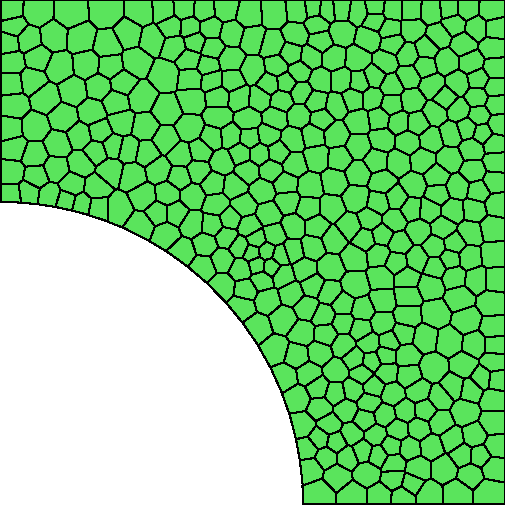
\includegraphics[width=0.5\textwidth]{../figures/voronoi_quad_circle.pdf}
%        \caption{多边形网格}
%    \end{figure}
%
%    \begin{figure}[htpb]
%        \centering
%        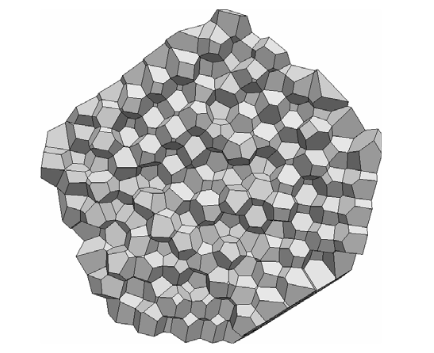
\includegraphics[width=0.6\textwidth]{../figures/polyhedron.png}
%        \caption{多面体网格}
%    \end{figure}
%\end{minipage}
%\end{frame}
\begin{frame}\frametitle{Poisson 方程}
\begin{minipage}[b]{0.6\linewidth}
考虑多边形 $\Omega$ 上的 Poisson 方程问题:
$$
\left\{
\begin{aligned}
-\Delta u &= f \quad \text{in} \quad \Omega, \\
u &= 0 \quad \text{on} \quad \partial \Omega,
\end{aligned}
\right.
$$
其中 $f \in L^2(\Omega)$。其对应的变分问题为:寻找 $u \in H^1_0(\Omega)$,使得
$$
a(u, v) = (f, v) \quad \forall v \in H^1_0(\Omega),
$$
其中 
$$
a(u, v) = \int_{\Omega} \nabla u \cdot \nabla v \, \mathrm{d} x
$$
\end{minipage}
\hfill
\begin{minipage}[b]{0.38\linewidth}
    \centering
    \begin{figure}[htpb]
        \centering
        
\includegraphics[width=0.65\textwidth]{../figures/domain_quad.pdf}
        \caption{多边形区域 $\Omega$}
    \end{figure}
\end{minipage}

\end{frame}

\begin{frame}
\frametitle{Poison 方程的线性有限元方法}
\begin{minipage}[b]{0.6\linewidth}
\begin{itemize}
\item 将 $\Omega$ 三角剖分为 $\mathcal{T}_h$。
\item 建立有限元空间 $V_h$:
    $$
    V_h = \{v_h \in H^1(\Omega): v_h|_K \in \mathbb{P}_1(K), \forall K \in
    \mathcal{T}_h\}.
    $$
\item 求解有限元问题:寻找 $u_h \in V_h$,使得
    $$
    a_h(u_h, v_h) = (f, v_h) \quad \forall v_h \in V_h,
    $$
    其中
    $$
    a_h(u_h, v_h) = \sum_{K \in \mathcal{T}_h} \int_K \nabla u_h \cdot \nabla v_h \,
    \mathrm{d} x
    $$
\end{itemize}
\vspace{15pt}
\end{minipage}
\hfill
\begin{minipage}[b]{0.38\linewidth}
    \begin{figure}[htpb]
        \centering
        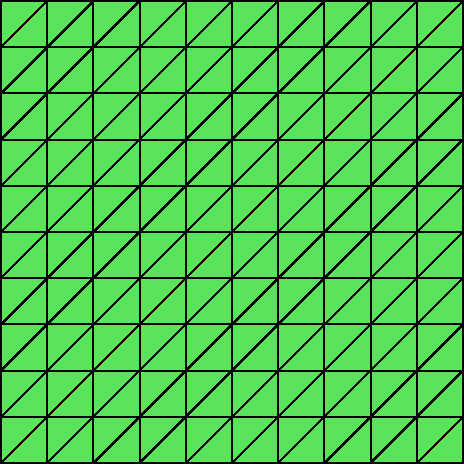
\includegraphics[width=0.5\textwidth]{../figures/struct_triangle_mesh.pdf}
        \caption{三角剖分}
    \end{figure}
    \begin{figure}[htpb]
        \centering
        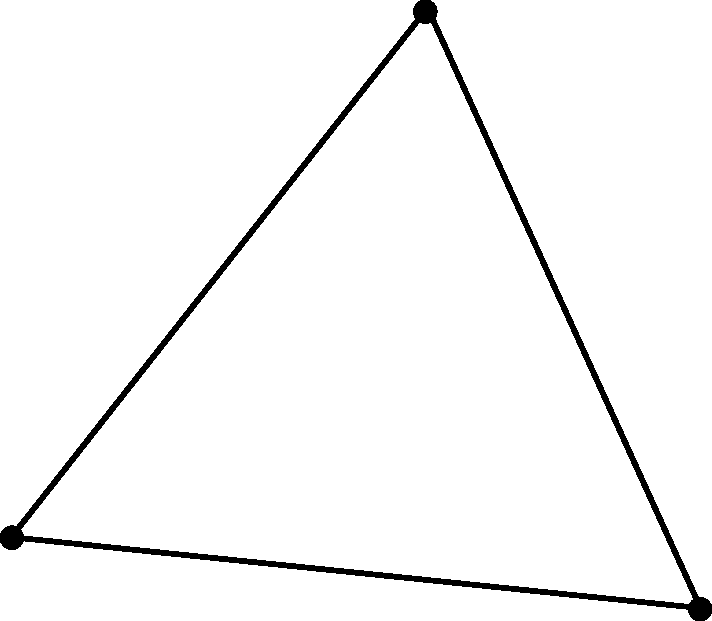
\includegraphics[width=0.4\textwidth]{../figures/triangle.pdf}
        \caption{三角形 $K$}
    \end{figure}
\end{minipage}
\end{frame}

\begin{frame}
    \frametitle{Poison 方程的虚单元方法}
\begin{minipage}[b]{0.6\linewidth}
\only<1>{
\begin{itemize}
\item 将 $\Omega$ 剖分为多边形网格 $\mathcal{T}_h$,
\item 建立虚单元空间 $V_h$:
$$
V_h = \{v_h \in H^1(\Omega): v_h|_K \in V_h^K, \forall K \in
\mathcal{T}_h\}.
$$
其中的 $V_h^K$ 为:
$$
V_h^K = \{v \in H^1(K): v|_{\partial K} \in \mathbb{P}_k(\partial K)
\Delta v = 0\}.
$$
\item 求解虚单元问题:寻找 $u_h \in V_h$,使得
$$
a_h(u_h, v_h) = (f, \Pi_hv_h) \quad \forall v_h \in V_h,
$$
\end{itemize}
\vspace{30pt}
}
\only<2>{
离散双线性型 $a_h$ 定义如下:
$$
a_h(u_h, v_h) = \sum_{K \in \mathcal{T}_h} a_h^K(u_h, v_h) 
$$
其中
$$
\begin{aligned}
a_h^K(u_h, v_h) = & \int_K \nabla \Pi_h^K u_h \cdot \nabla \Pi_h^K v_h \, \mathrm{d}
x\\
& + \marking{S_h^K(u_h - \Pi_h^K u_h, v_h - \Pi_h^K v_h)}.
\end{aligned}
$$
\vspace{40pt}
}
\end{minipage}
\hfill
\begin{minipage}[b]{0.38\linewidth}
    \centering
    \begin{figure}[htpb]
        \centering
        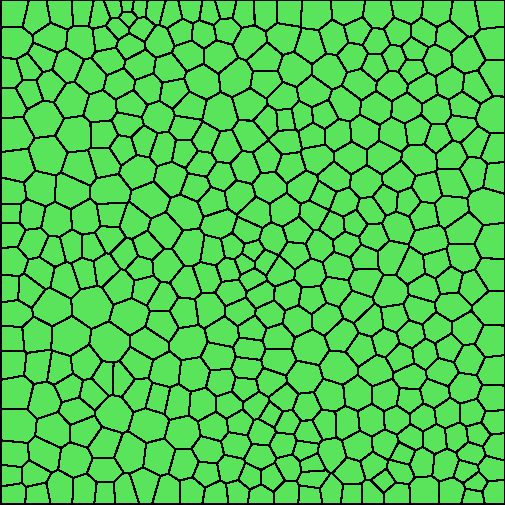
\includegraphics[width=0.6\textwidth]{../figures/voronoi_quad.pdf}
        \caption{多边形网格}
    \end{figure}
    \begin{figure}[htpb]
        \centering
        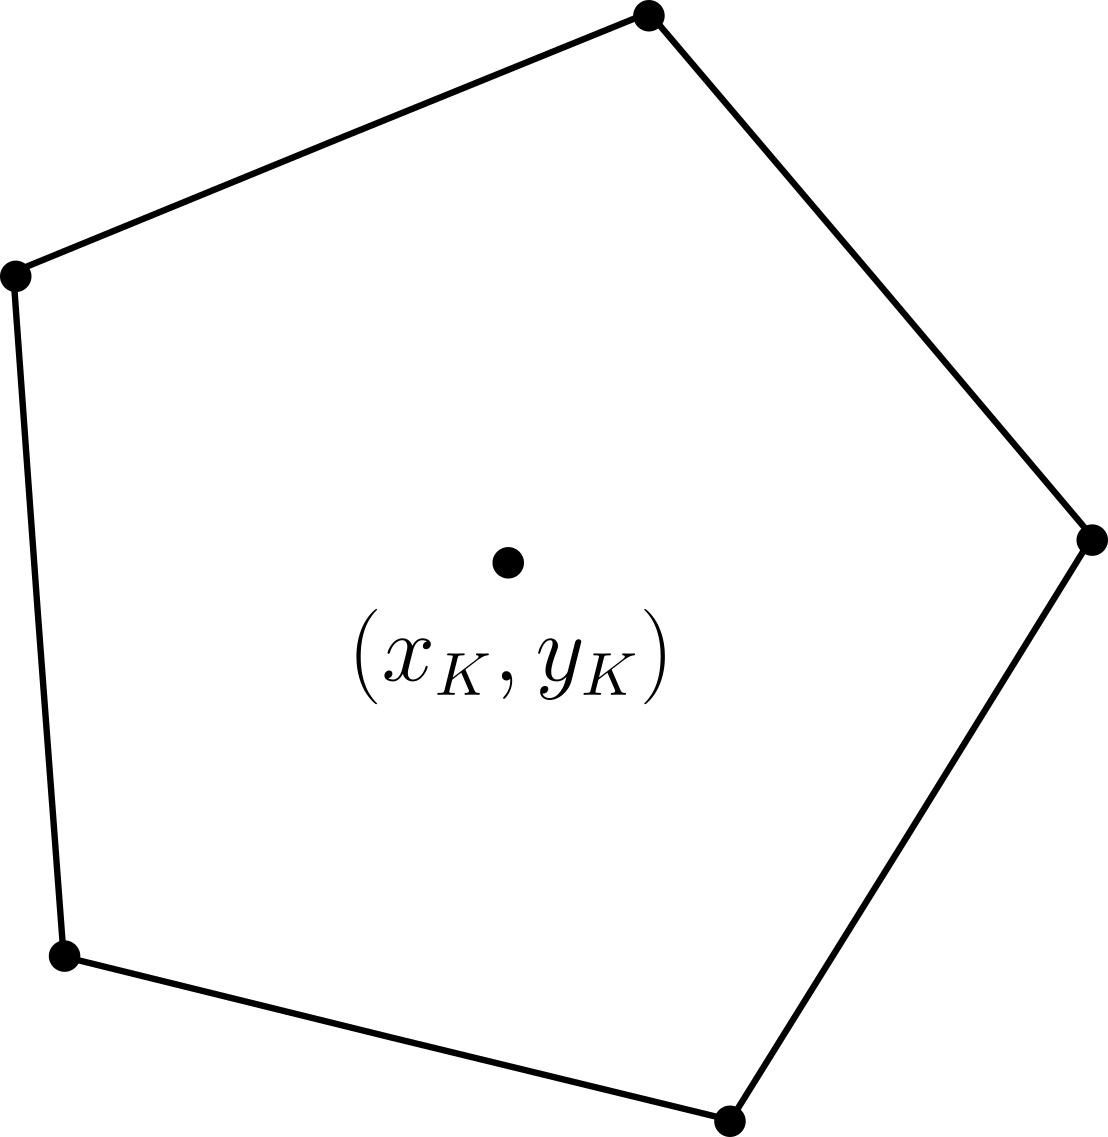
\includegraphics[width=0.5\textwidth]{../figures/polygon_K.png}
        \caption{多边形 $K$}
    \end{figure}
\end{minipage}
\end{frame}

\begin{frame}
    \frametitle{虚单元方法的优缺点}
\begin{minipage}[b]{0.6\linewidth}
\textbf{优点:}
\begin{itemize}
    \item \textbf{灵活性}:可以在任意多边形网格上计算。
    \item \textbf{单元函数光滑性低}:方便于定义更好正则性的虚单元空间。
\end{itemize}
\vspace{10pt}
\textbf{缺点:}
\begin{itemize}
    \item \textbf{实现复杂}:相比于有限元,虚单元实现更为复杂。 
    \item \textbf{稳定化项}:在非线性问题中,系数的选取对数值结果有较大影响。
\end{itemize}
\end{minipage}
\hfill
\begin{minipage}[b]{0.38\linewidth}
    \centering
    \begin{figure}[htpb]
        \centering
        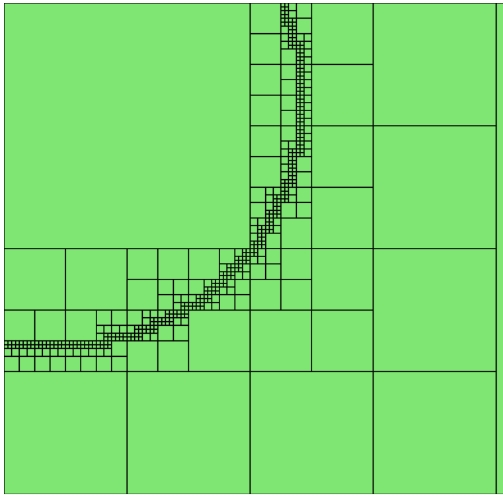
\includegraphics[width=0.65\textwidth]{../figures/four.jpg}
        \caption{四叉树网格}
    \end{figure}
\end{minipage}
\end{frame}
\section{任意维任意 $H^m$ 协调的虚单元空间}
\begin{frame}
  \frametitle{$H^m$ 协调性}
  \begin{lemma}[Green' identity]
      Let $K\in\mathbb{R}^n$, for any $v \in H^m(K)$ and $q \in H^{2m}(K)$:
      $$
      (\nabla^m v, \nabla^m q)_K = (v, (-\Delta)^m q) + \sum_{i=0}^{m-1}
      (\nabla^i v, \nabla^i(-\Delta)^{m-i-1}\partial_{\boldsymbol{\nu}}q)_{\partial K}
      $$
  \end{lemma}
  Let $\nabla_F  = \sum_{i}\boldsymbol{t}_{F, i}
  \frac{\partial v}{\partial \boldsymbol{t}_{F, i}}$, then $\nabla = \nabla_F +
  \boldsymbol{\nu}_F \frac{\partial }{\partial \boldsymbol{\nu}_F}$
  %\begin{itemize}
  %    \item $(\nabla^m v)|_F$ is continues $\Longleftrightarrow
  %        (\frac{\partial^l v}{\partial \boldsymbol{\nu}_F^l})|_F$ is continues.
  %\end{itemize}
  $$
  \begin{aligned}
  (\nabla^m v, \nabla^m q)_K
  & = (v, (-\Delta)^m q)_K + \sum_{i=0}^{m-1}
     \sum_{l=0}^i\sum_{F\in\mathcal{F}^1(K)}
     \left(\frac{i!}{l!(i-l!)}\right)^2
     \\
     & \quad\quad\quad\quad\quad(\nabla^{l}_{F}\partial^{i-l}_{\boldsymbol\nu_F} v,
     \nabla^{l}_{F}
     (-\Delta)^{m-i-1}\partial^{i-l+1}_{\boldsymbol\nu_F}q)_F\\
  \end{aligned}
  $$
  \begin{itemize}
      \item $H^m$ 协调性 $\Longleftrightarrow$ $m-1$ 阶法向导数连续。
  \end{itemize}
\end{frame}

\begin{frame}
  \frametitle{$H^m$ conforming}
  If $v \in H^m(K_1)$ and $v \in H^m(K_2)$, then:\\
  \vspace{0.5cm}
  \centering
  $v \in H^m(K_1\cap K_2) \Longleftrightarrow  
  (\frac{\partial^l v}{\partial \boldsymbol{\nu}_F^l})|_F$ is continues.

  \begin{figure}[H]
    \centering
    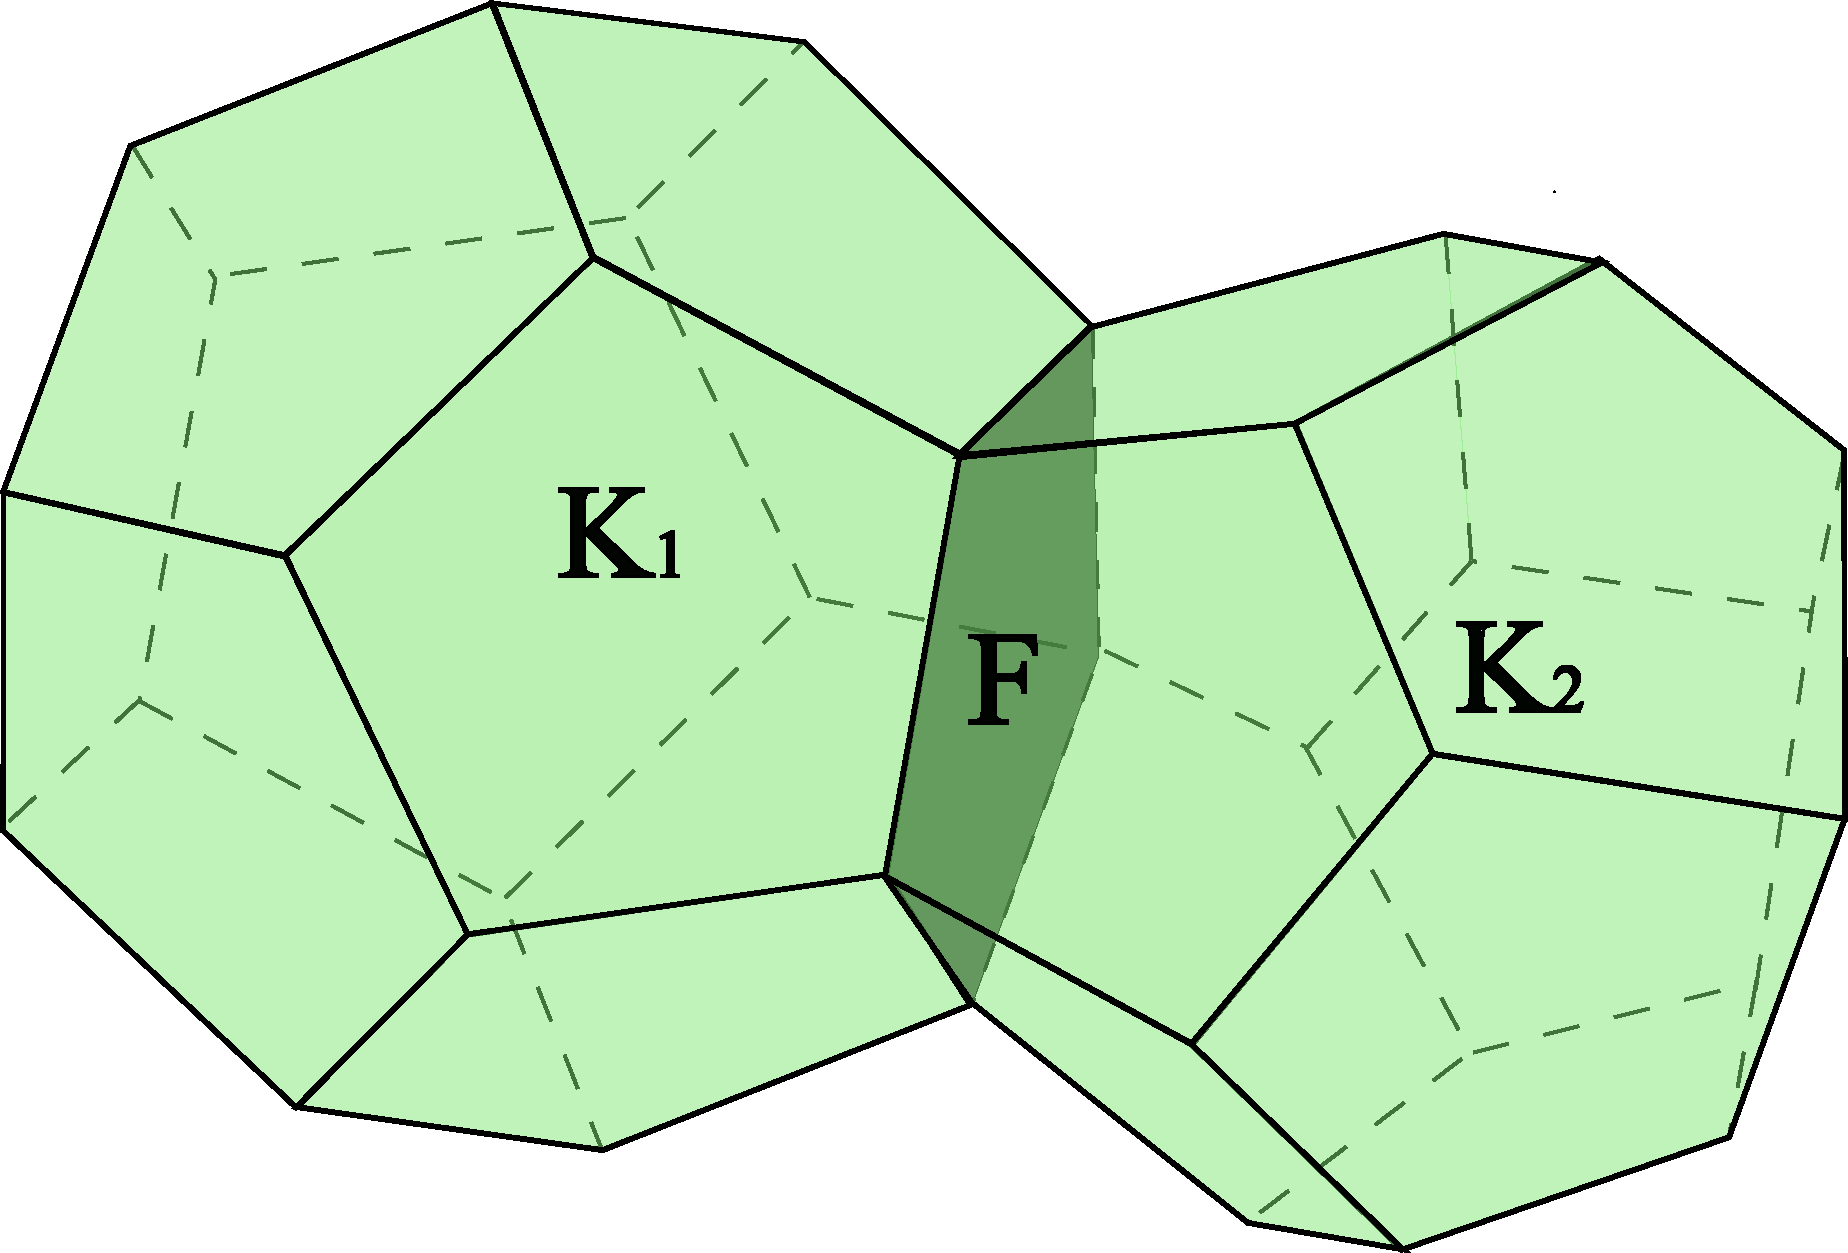
\includegraphics[scale=0.2]{../figures/dodecahedron.pdf}
  \end{figure} 
\end{frame}


\begin{frame}
\frametitle{$H^m$-Conforming virtual element in $\mathbb{R}^1$}
Let $K$ is an interval, \bf{DoFs}:
\begin{itemize}
    \item $h_K^j v^{(j)}(\delta) \quad \forall \delta \in \mathcal{F}^1(K),
        j = 0, 1, \dots, m-1$,
    \item $\frac{1}{|K|}(v, q)_K \quad \forall q \in \mathbb{P}_{k-2m}(K)$. 
\end{itemize}
\bf{shape function space}:
$$
V_k^m(K) := \{v \in H^m(K): v^{(2m)}\in\mathbb{P}_{k-2m}(K)\} = 
\left\{ 
\begin{aligned}
    \mathbb{P}_{k} \quad & k\geq 2m-1\\
    \mathbb{P}_{2m-1} \quad & k < 2m-1
\end{aligned}
\right.
$$
\end{frame}

\begin{frame}
\frametitle{$H^m$-Conforming virtual element in $\mathbb{R}^2$}
Let $K$ is a polygon, define a preliminary space:
$$
\small{
\begin{aligned}
  \widetilde{V}_k^m(K) := \Big\{v \in H^m(K) : & (-\Delta)^m v \in P_k(K),\\ 
      & \frac{\partial^j v}{\partial \boldsymbol{\nu}_e^j} \in V_{k-j}^{m-j}(e) \quad 
    \forall e \in \mathcal{F}^1(K), j=0, 1, \dots, m-1\Big\}.
\end{aligned}
}
$$
\begin{itemize}
    \item $\mathbb{P}_k(K) \subseteq \widetilde{V}_k^m(K)$ but 
        $\mathbb{P}_{k+1}(K) \not\subseteq \widetilde{V}_k^m(K)$.
    \item $\nabla^j v$ is continuous on $\partial K$.
\end{itemize}

\bf{Choose DoFs as}:
\begin{itemize}
    \item $h_K^j \nabla^{j}v(\delta) \quad \forall \delta \in \mathcal{F}^2(K),
        j = 0, 1, \dots, m-1$,
    \item $\frac{h_K^j}{|e|}(\frac{\partial^j v}{\partial \boldsymbol{\nu}_e^j}, q) \quad 
        \forall q \in \mathbb{P}_{k-2m+j}(e), e \in \mathcal{F}^1(K), 
        j = 0, 1, \dots, m-1$,
    \item $\frac{1}{|K|}(v, q)_K \quad \forall q \in \mathbb{P}_{k-2m}(K)$. 
\end{itemize}
\end{frame}

\begin{frame}
\frametitle{$H^m$-Conforming virtual element in $\mathbb{R}^2$}
    \textbf{shape function space as}:
    $$
    V_k^m(K) := \{v \in \widetilde{V}_k^m(K): (v, q) = (\Pi_k^Kv, q) \quad 
        \forall q \in \mathcal{P}_{k-2m}^{\perp}(K)\}
    $$
    where $\Pi_k^K : \widetilde{V}_k^m(K) \to \mathbb{P}_k(K)$ defined as:
    $$
    \begin{aligned}
        (\nabla^m \Pi_k^K v, \nabla^m q) &  = (\nabla^m v, \nabla^m q) \quad
        \forall q \in \mathbb{P}_k(K)\\
        \sum_{\delta\in\mathcal{F}^2(K)}(\nabla^j\Pi_k^K v)(\delta) & = 
        \sum_{\delta\in\mathcal{F}^2(K)}(\nabla^j v)(\delta) \quad j = 0, 1,
        \dots, m-1.
    \end{aligned}
    $$
    Let $Q_k^K : \widetilde{V}_k^m(K) \to \mathbb{P}_k(K)$ is $L^2$ projection
    then:
    $$
    Q_k^K = \Pi_k^K + Q_{k-2m} - Q_{k-2m}\Pi_k^K 
    $$
\end{frame}
\begin{frame}
    \frametitle{通过粘贴构造 $H^m$-Conforming 虚单元空间}
    \begin{figure}[H]
        \centering
        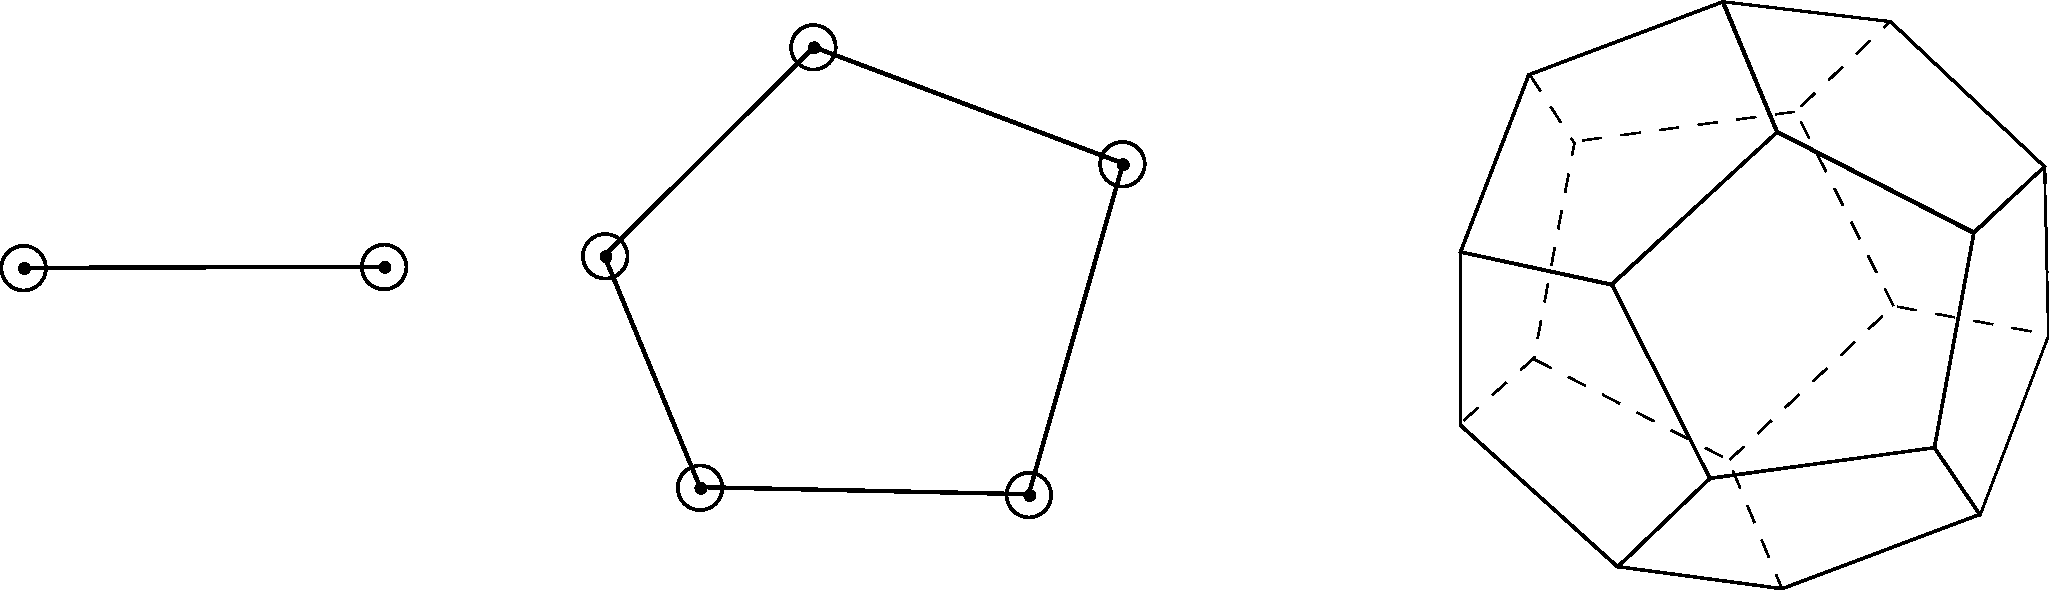
\includegraphics[scale=0.3]{../figures/bitmap.pdf}
    \end{figure}
\end{frame}

\begin{frame}
    \frametitle{$H^m$-Conforming virtual element in $\mathbb{R}^n$}
    Let $K \subset \mathbb{R}^n$ is a polytope, define a preliminary space:
    $$
    \small{
    \begin{aligned}
      \widetilde{V}_k^m(K) := \Big\{v \in  H^m(K) :&  (-\Delta)^m v \in P_k(K),\\
          & \nabla^j v|_{\mathcal{S}^r(K)} \in H^1(\mathcal{S}^r(K),\mathbb{S}_n(j)), \\
          & \qquad\qquad j = 0, 1, \dots, m-1, r = 1, 2, \dots, n\\
          & \frac{\partial^j v}{\partial
          \boldsymbol{\nu}_F^{\boldsymbol{\alpha}}} \in V_{k-j}^{m-j}(F) \quad 
          \forall F \in \mathcal{F}^r(K), \\
          &\qquad\qquad r = 1, 2, \dots, n-1, \boldsymbol{\alpha} \in \mathcal{A}_{m-1}^r.
          \Big\}
    \end{aligned}
    }
    $$
    \begin{itemize}
        \item $\mathbb{P}_k(K) \subseteq \widetilde{V}_k^m(K)$ but 
            $\mathbb{P}_{k+1}(K) \not\subseteq \widetilde{V}_k^m(K)$.
    \end{itemize}
\end{frame}
\begin{frame}
    \frametitle{$H^m$-Conforming virtual element in $\mathbb{R}^n$}
    \textbf{Choose DoFs as} $\mathcal{N}_k^m(K)$:
  \begin{itemize}
    \item $h_K^j\nabla^{j}v(\delta) \quad\forall~\delta\in\mathcal F^{n}(K),\;
         j=0,1,\cdots,m-1,$
    \item $\frac{h_K^{j}}{|F|}(
        \frac{\partial^{\boldsymbol{\alpha}}v}{\partial
    \boldsymbol{\nu}_F^{\boldsymbol{\alpha}}}, q)_F
        \quad\forall~q\in\mathbb P_{k-2m+j}(F), F\in\mathcal
        F^{r}(K),$\\
        $\quad\quad\quad\quad\quad\quad
        \boldsymbol{\alpha}\in \mathcal{A}_j^r, 
        r = 1, 2, \dots, n-1, j=0,1,\cdots,m-1$
    \item $\frac{1}{|K|}(v, q)_K \quad\forall~q\in\mathbb P_{k-2m}(K)$ 
  \end{itemize}
  \textbf{shape function space as}:
    $$
    V_k^m(K) := \{v \in \widetilde{V}_k^m(K): (v, q) = (\Pi_k^Kv, q) \quad 
        \forall q \in \mathcal{P}_{k-2m}^{\perp}(K)\}
    $$
where $\Pi_k^K : \widetilde{V}_k^m(K) \to \mathbb{P}_k(K)$ defined as:
$$
\begin{aligned}
    (\nabla^m \Pi_k^K v, \nabla^m q) &  = (\nabla^m v, \nabla^m q) \quad
    \forall q \in \mathbb{P}_k(K)\\
    \sum_{\delta\in\mathcal{F}^2(K)}(\nabla^j\Pi_k^K v)(\delta) & = 
    \sum_{\delta\in\mathcal{F}^2(K)}(\nabla^j v)(\delta) \quad j = 0, 1,
    \dots, m-1.
\end{aligned} 
$$
\end{frame}

\begin{frame}
    \frametitle{VEM VS FEM}
\begin{minipage}[b]{0.49\linewidth}
    \large{\textbf{FEM}}:
    \begin{itemize}
        \item Include super-smooth DoFs.
        \item Requires a polynomial degree of at least $2^n \times (m-1)
            +1$.
    \end{itemize}
    \hfill \\
\end{minipage}
\hfill
\begin{minipage}[b]{0.49\linewidth}
    \large{\textbf{VEM}}:
    \begin{itemize}
        \item Does not include super-smooth DoFs.
        \item Require a polynomial degree only greater than $m$
        \item If $k = m$, the Dofs are $\nabla^j v(\delta), j < m$.
    \end{itemize}
\end{minipage}
\end{frame}

\begin{frame}
\frametitle{Polyharmonic equation}

\begin{definition}[Polyharmonic equation]
  Let $\Omega = (0, 1)\times(0, 1)$, Consider polyharmoic equation:
  $$
  \left\{
  \begin{aligned}
      (-\Delta)^m u + c u & = f \quad \Omega\\
      \frac{\partial^j u}{\partial \boldsymbol{\nu}^j} & = 0 \quad \partial\Omega,
      j = 0, 1, \dots, m-1.
  \end{aligned}
  \right.
  $$
\end{definition}
\begin{definition}[Variational form]
Find $u\in H_0^m(\Omega)$ such that
$$
(\nabla^mu, \nabla^mv)+c(u, v)=(f, v)\quad\forall~v\in H_0^m(\Omega),
$$
where $f\in L^2(\Omega)$ and constant $c\geq0$.
\end{definition}
\hspace*{\fill} \\
\hspace*{\fill} \\
\hspace*{\fill} \\
\hspace*{\fill} \\
\hspace*{\fill} \\
\end{frame}

\note[itemize]{
\item 
    \begin{CJK}{UTF8}{gkai}
        $H^m$ 协调元的一个直接应用就是多重调和方程,
        我们考虑这样一个带有低阶项的多重调和方程, 他的变分形式就是下面这样.
    \end{CJK}
\item A direct application of $H^m$ conforming elements is in the context of
    polyharmonic equations. Consider a polyharmonic equation with lower-order
    terms, this is its variational form.
}

\begin{frame}
\begin{definition}[VEM for polyharmonic equation]
  Let $\mathcal{T}_h$ is a polytope mesh on $\Omega$, 
  define the virtual element space:
  $$
  V_h:=\{v_h\in H_0^m(\Omega): v_h|_K\in V_{k}^{m}(K) \textrm{ for each } K\in\mathcal T_h\}.
  $$
  The VEM of polyharmonic equation is that: {\bf find $u_h \in V_h$ statify}: 
  $$
  a_{h}(u_h, v_h)=\langle f, v_h\rangle\quad\forall~v_h\in V_h,
  $$
  {\bf where} $\langle f, v_h\rangle:=\sum\limits_{K\in\mathcal T_h}(f,
  Q_k^Kv_h)_K, a_h(u_h, v_h):=\sum_{K\in\mathcal T_h}a_{h,K}(u_h, v_h),$
  $$
  \begin{aligned}
  a_{h,K}(u_h, v_h):=&\,(\nabla^m\Pi_k^Ku_h,
  \nabla^m\Pi_k^Kv_h)_K+S_K(u_h-\Pi_k^Ku_h,v_h-\Pi_k^Kv_h) \\
  &+c(Q_k^Ku_h, Q_k^Kv_h)_K.
  \end{aligned}
  $$
\end{definition}
\hspace*{\fill} \\
\hspace*{\fill} \\
\hspace*{\fill} \\
\end{frame}

\begin{frame}
  \frametitle{Stablized term}
  \begin{definition}[Stablized term]
    \footnotesize{
    $$
    S_K(w,v):=\sum_{r=1}^{n}\sum_{F\in\mathcal F^{r}(K)}\sum_{\alpha\in A_{r}\atop
    |\alpha|\leq
    m-1}h_K^{r+2|\alpha|-2m}\bigg(Q_{k-2m+|\alpha|}^{F}\frac{\partial^{|\alpha|}w}{\partial
    \boldsymbol{\nu}_{F}^{\alpha}},Q_{k-2m+|\alpha|}^{F}\frac{\partial^{|\alpha|}v}{\partial
    \boldsymbol{\nu}_{F}^{\alpha}}\bigg)_{F}
    $$
  }
  \end{definition}
  \begin{lemma}
      $$
      S_K(v-\Pi_k^Kv,v-\Pi_k^Kv)\eqsim |v-\Pi_k^Kv|_{m,K}^2\quad\forall~v\in V_{k}^{m}(K).
      $$
  \end{lemma}
    \begin{lemma}
    $$
    a_{h,K}(w, v)\lesssim (|w|_{m,K}+\|w\|_{0,K})(|v|_{m,K}+\|v\|_{0,K})\quad\forall~w,v\in V_{k}^{m}(K),
    $$
    $$
    a_{h}(v_h, v_h)\eqsim |v_h|_{m}^2\quad\forall~v_h\in V_h.   
    $$
    \end{lemma}
\end{frame}


\begin{frame}
\frametitle{Error estimate}
\begin{theorem}\label{errorestimate}
Let $u\in H^s(\Omega)\cap H_0^m(\Omega)$ with $s\geq m$ be the solution of the
polyharmonic equation, and $u_h\in V_h$ be the solution
of the conforming virtual element method. Assume the mesh. Assume
$f\in H^m(\mathcal T_h)$. Then we have
$$
|u-u_h|_m\lesssim h^{\min\{s,k+1\}-m}|u|_{\min\{s,k+1\}}+\textrm{osc}_h(f),
$$
$$
|u-\Pi_hu_h|_{m,h}\lesssim h^{\min\{s,k+1\}-m}|u|_{\min\{s,k+1\}}+\textrm{osc}_h(f),
$$
where $\textrm{osc}_h^2(f):=\sum\limits_{K\in\mathcal T_h}h_K^{2m}\|f-Q_k^Kf\|_{0,K}^2$.
\end{theorem}

\end{frame}

\begin{frame}
  \frametitle{Biharmonic equation}
  Let $\Omega = (0, 1)\times(0, 1)$, Consider biharmoic equation:
  $$
  \left\{
  \begin{aligned} 
      \Delta^2 u + 2u & = f \quad \Omega\\
      \frac{\partial^j u}{\partial \boldsymbol{n}^j} & = 0 \quad \partial\Omega,
      j = 0, 1.
  \end{aligned}
  \right.
  $$
  with true solution $u = \sin^2(\pi x)\sin^2(\pi y)$.

\begin{figure}[htb p]
\centering
\begin{minipage}[t]{0.49\linewidth}
\centering
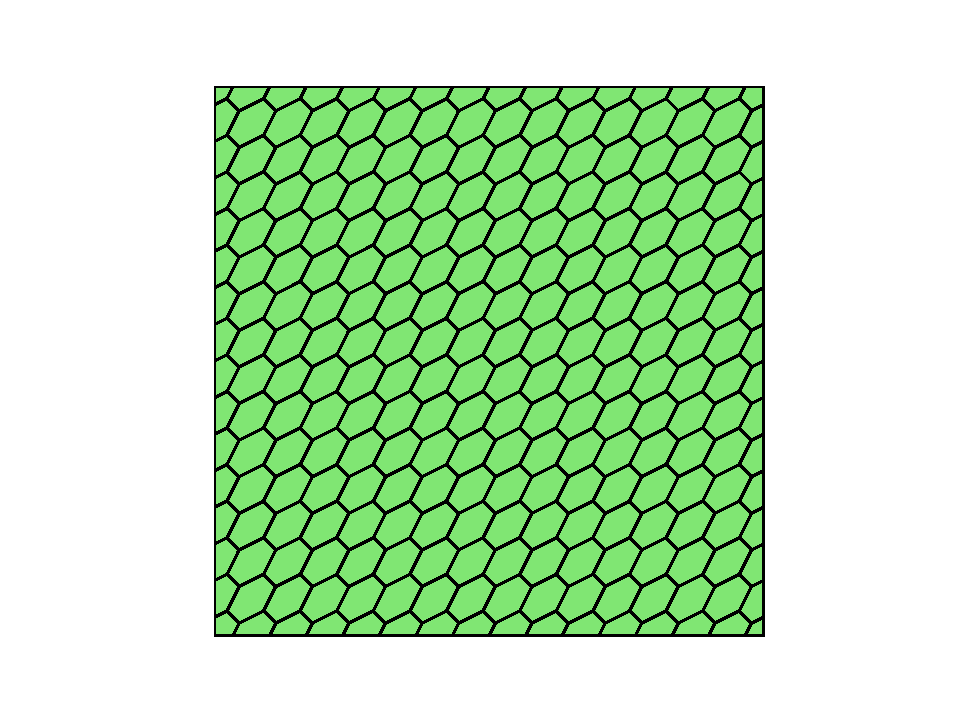
\includegraphics[width=4cm]{../figures/convex.pdf}
\captionsetup{font={small}}
\caption{Convex polygon mesh $\mathcal T_0$}
\end{minipage}%
\begin{minipage}[t]{0.49\linewidth}
\centering
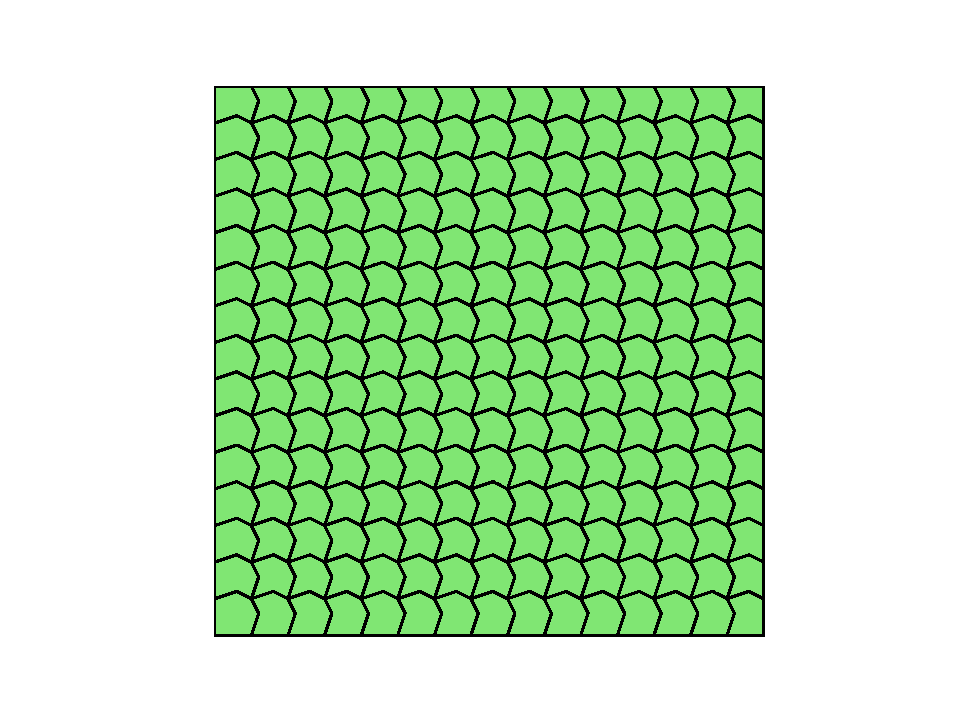
\includegraphics[width=4cm]{../figures/nonconvex.pdf}
\captionsetup{font={small}}
\caption{Non-convex polygon mesh $\mathcal T_1$}
\end{minipage}%
\centering
%\caption{\small Convex polygon mesh $\mathcal T_0$(left) and non-convex polygon mesh 
%$\mathcal T_1$(right).}
\label{fig:mesh}
\end{figure}
\end{frame}

\begin{frame}
  \frametitle{Numberical result of VEM}
\begin{figure}[htbp]
\centering
\begin{minipage}[t]{0.49\linewidth}
\centering
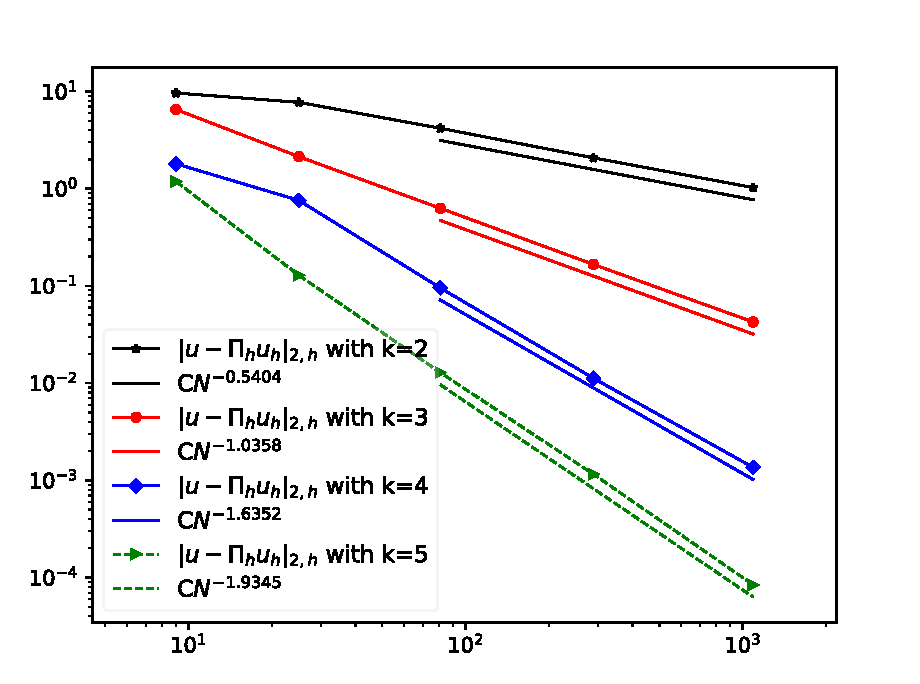
\includegraphics[width=5cm]{../figures/H2_convex.pdf}
%\caption{Numberical result of example with $\mathcal T_0$.}
\end{minipage}%
\begin{minipage}[t]{0.49\linewidth}
\centering
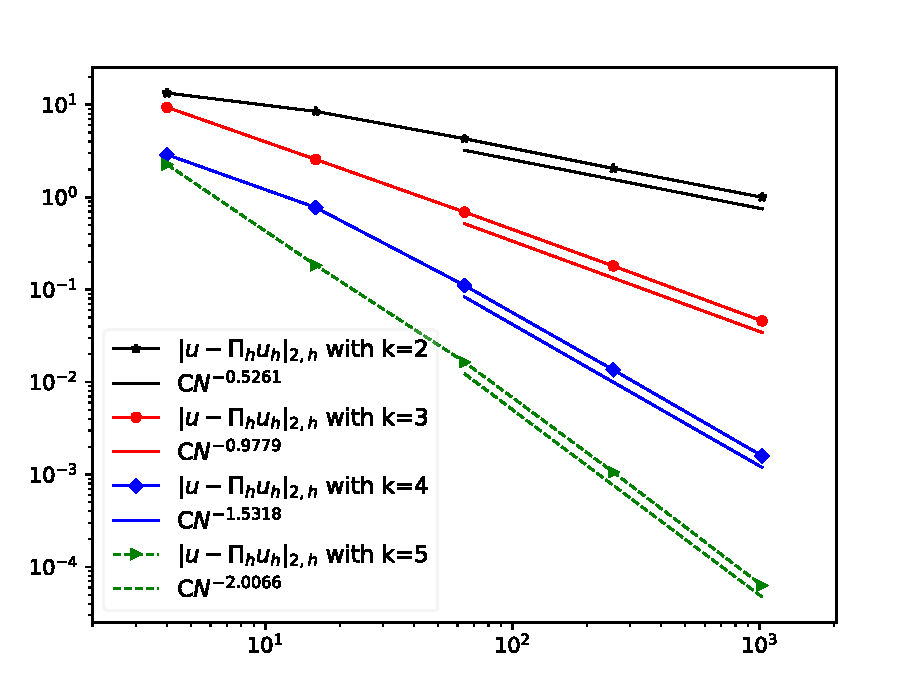
\includegraphics[width=5cm]{../figures/H2_nonconvex.pdf}
%\caption{[Numberical result of example with $\mathcal T_1$].}
\end{minipage}%
\centering
\caption{Error $|u - \Pi_h u_h|_{2, h}$ of biharmonic 
    equation with $m=2$ on convex polygon mesh $\mathcal T_0$(left) 
and non-convex polygon mesh $\mathcal T_1$(right) with $k = 2, 3, 4, 5$.}
\label{fig:H2error}
\end{figure} 
\end{frame}

\begin{frame}
  \frametitle{Triharmonic equation}
  Let $\Omega = (0, 1)\times(0, 1)$, Consider triharmoic equation:
  $$
  \left\{
  \begin{aligned}
      -\Delta^3 u + 2u & = f \quad \Omega\\
      \frac{\partial^j u}{\partial \boldsymbol{n}^j} & = 0 \quad \partial\Omega,
      j = 0, 1, 2.
  \end{aligned}
  \right.
  $$
  with true solution $u = \sin^3(\pi x)\sin^3(\pi y)$.

\begin{figure}[htbp]
\centering
\begin{minipage}[t]{0.49\linewidth}
\centering
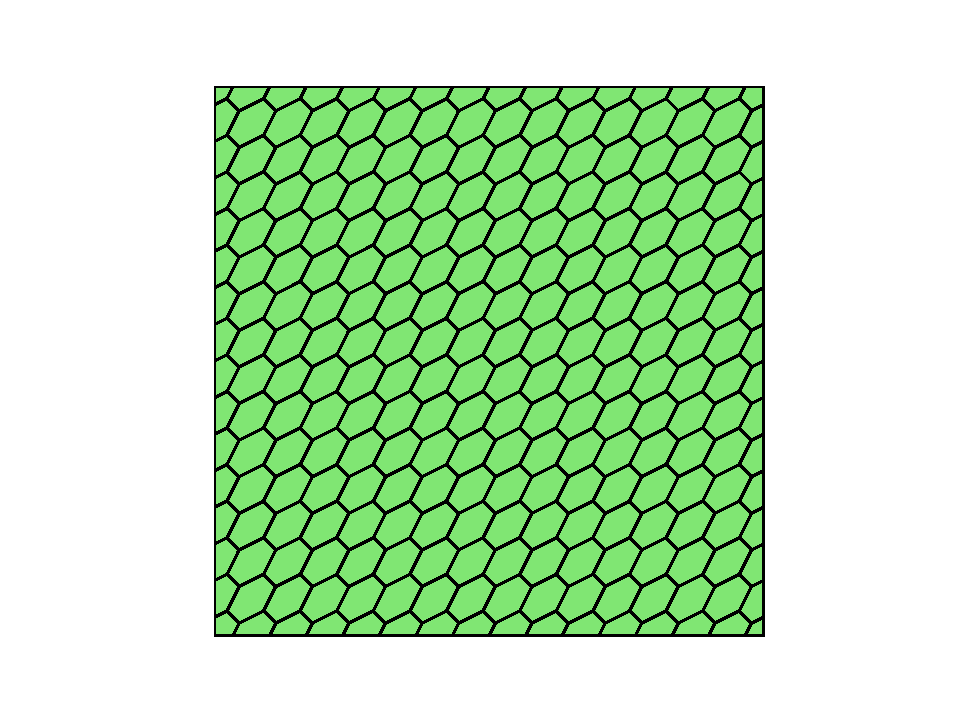
\includegraphics[width=4cm]{../figures/convex.pdf}
\captionsetup{font={small}}
\caption{Convex polygon mesh $\mathcal T_0$}
\end{minipage}%
\begin{minipage}[t]{0.49\linewidth}
\centering
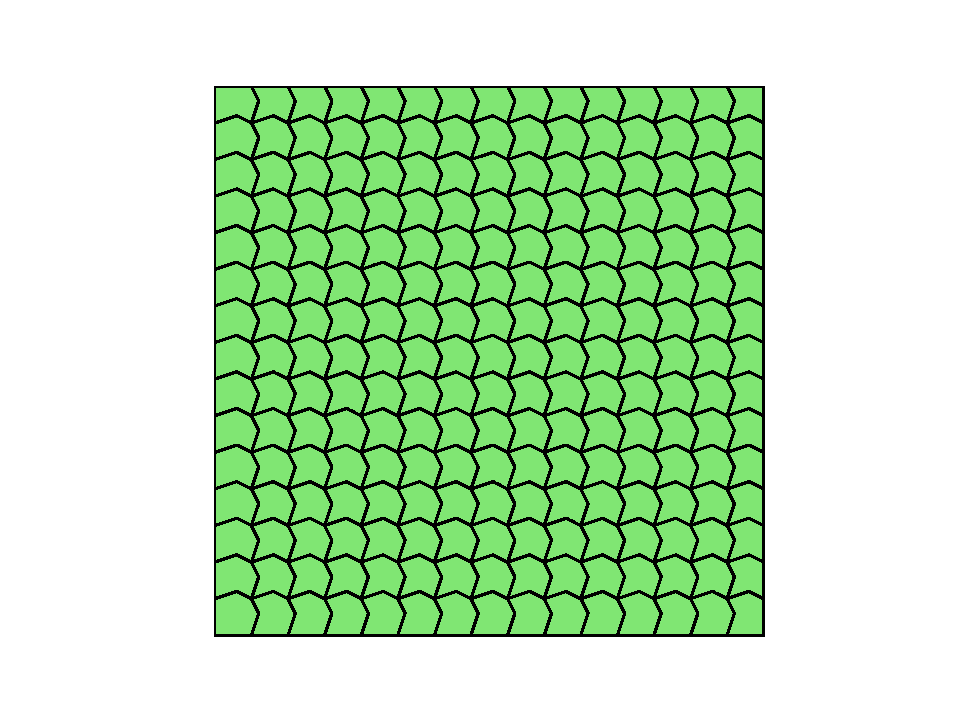
\includegraphics[width=4cm]{../figures/nonconvex.pdf}
\captionsetup{font={small}}
\caption{Non-convex polygon mesh $\mathcal T_1$}
\end{minipage}%
\centering
%\caption{\small Convex polygon mesh $\mathcal T_0$(left) and non-convex polygon mesh 
%$\mathcal T_1$(right).}
\label{fig:mesh}
\end{figure}

\end{frame}

\begin{frame}
  \frametitle{Numberical result of VEM}
\begin{figure}[htbp]
\centering
\begin{minipage}[t]{0.49\linewidth}
\centering
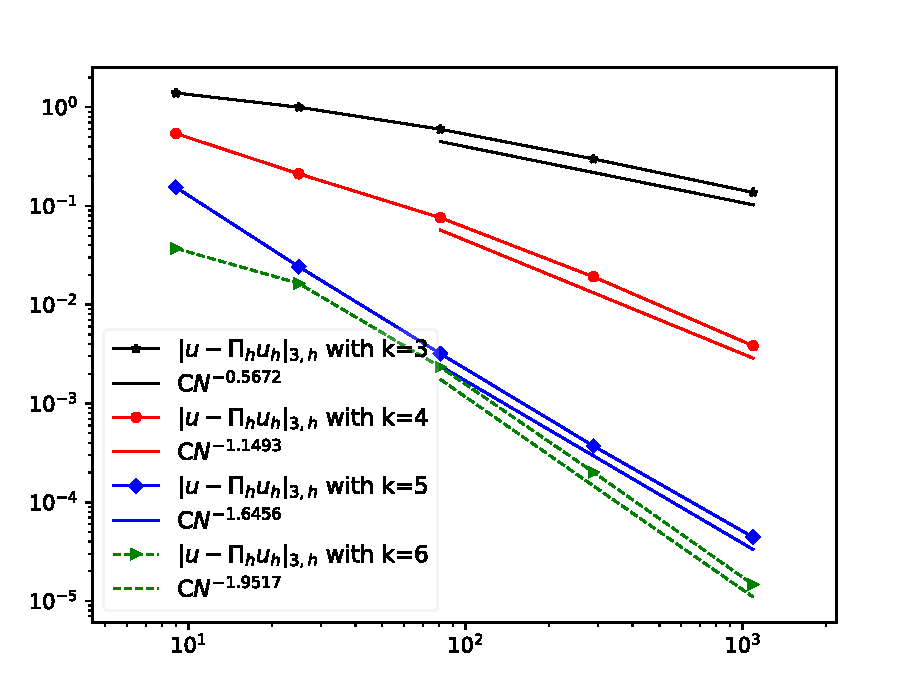
\includegraphics[width=5cm]{../figures/H3_convex.pdf}
%\caption{Numberical result of example with $\mathcal T_0$.}
\end{minipage}%
\begin{minipage}[t]{0.49\linewidth}
\centering
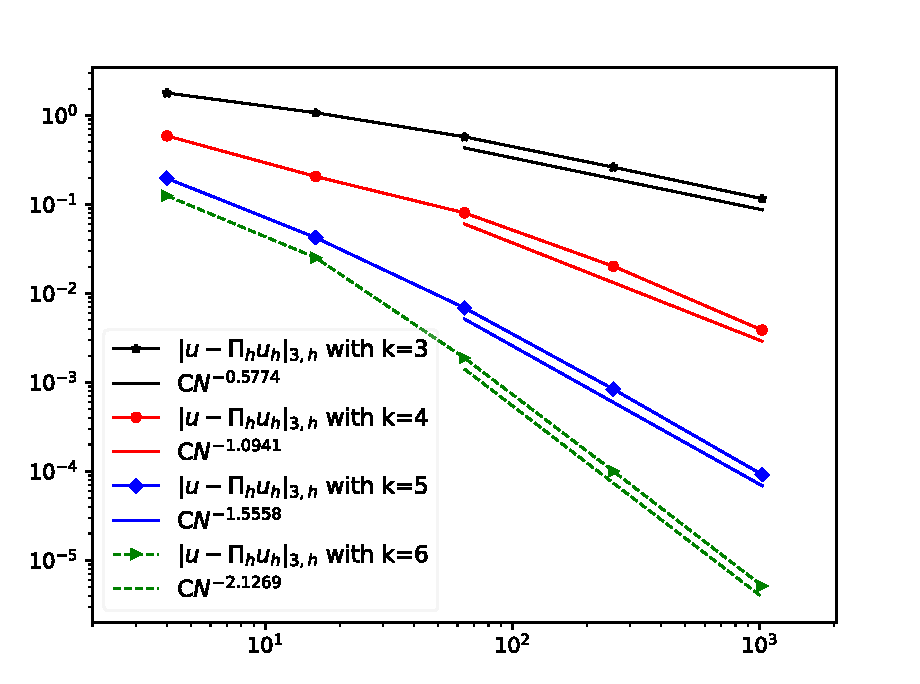
\includegraphics[width=5cm]{../figures/H3_nonconvex.pdf}
%\caption{[Numberical result of example with $\mathcal T_1$].}
\end{minipage}%
\centering
\caption{Error $|u - \Pi_h u_h|_{3, h}$ of 
    triharmonic equation with $m=3$ on convex polygon mesh $\mathcal T_0$(left) 
and non-convex polygon mesh $\mathcal T_1$(right) with $k = 3, 4, 5, 6$.}
\label{fig:H3error}
\end{figure}
\end{frame}
\section{无稳定子虚单元方法}
\begin{frame}
\frametitle{无稳定子虚单元方法}
  给定虚单元空间 $V_h$,Poison 方程的虚单元方法为:寻找 $u_h \in V_h$,使得
  $$
  a_h(u_h, v_h) = (f, v_h) \quad \forall v_h \in V_h,
  $$
  离散双线性型 $a_h$ 定义为:
  $$
  a_h(u_h, v_h) = \sum_{K \in \mathcal{T}_h} a_h^K(u_h, v_h)
  $$
  $$
  a_h^K(u_h, v_h) = \int_K \nabla \Pi_h^K u_h \cdot \nabla \Pi_h^K v_h \,
  \mathrm{d} x + \marking{S_h^K(u_h - \Pi_h^K u_h, v_h - \Pi_h^K v_h)}.
  $$
  稳定化项 $S_h^K$ 需满足:
  $$
  c_* |v|_{1, K}^2 \leq S_h^K(v, v) \leq C_* |v|_{1, K}^2 \quad \forall v \in 
  V_h^K \cap \mathrm{ker}(\Pi_h^K).
  $$
\end{frame}

\begin{frame}
\frametitle{无稳定子虚单元方法}
\begin{minipage}[b]{0.6\linewidth}
\uncover<1->{
\textbf{目标}: 找到一个合适的空间 $W_h^K$,使得
\begin{itemize}
    \item $\nabla V_h^K$ 到 $W_h^K$ 的投影 $Q^K$ 可以计算。
    \item $\|Q^k \nabla v\| \eqsim \|\nabla v\| \quad \forall v \in V_h^K$.
\end{itemize}
\vspace{10pt}
}
\uncover<2->{
\textbf{方法:}
将 $K$ 分成三角形网格 $\mathcal{T}_K$
在 $\mathcal{T}_K$ 上建立 k-BDM 元空间 $\tilde{W}_h^k$,定义 $W_h^K$ 为
$$
W_h^K = \{\boldsymbol{v} \in \tilde{W}_h^{k-1}: \mathrm{div} \boldsymbol{v} \in
\mathbb{P}_{k-2}(K)\}.
$$
那么:$\nabla V_h^K$ 到 $W_h^K$ 的 $L^2$ 正交投影 $Q^K$ 可以计算:
$$
\begin{aligned}
(Q^K \nabla\boldsymbol{v}, \boldsymbol{w})_K & = (\nabla v, \boldsymbol{w})_K\\
& = (v, \mathrm{div} \boldsymbol{w})_K + \langle v, \boldsymbol{w} \cdot 
\boldsymbol{n}\rangle_{\partial K}.
\end{aligned}
$$
}
\end{minipage}
\hfill
\begin{minipage}[b]{0.38\linewidth}
    \centering
    \uncover<2->{
    \begin{figure}[htpb]
        \centering
        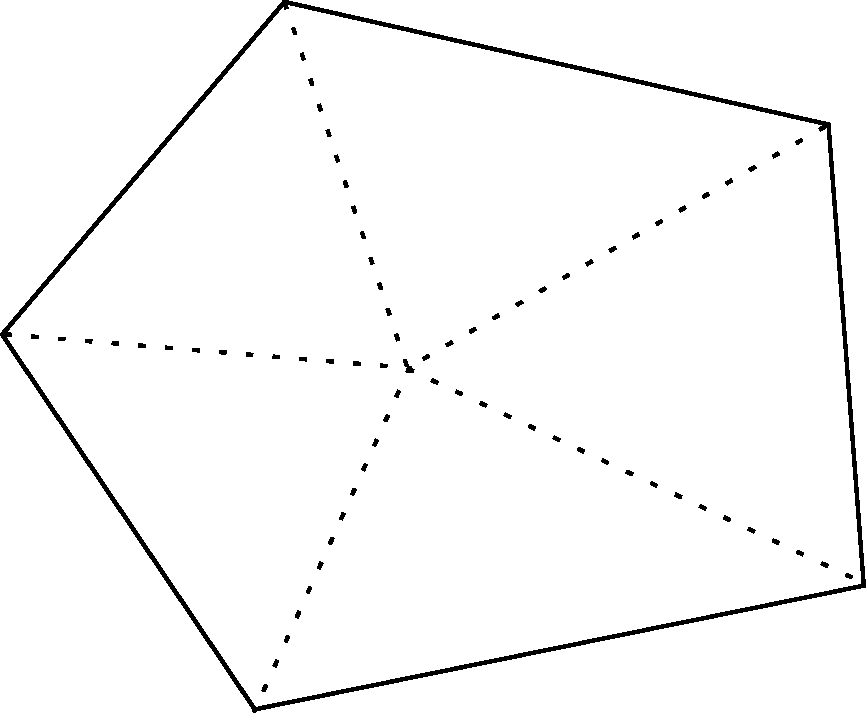
\includegraphics[width=0.8\textwidth]{../figures/splite_polygon.pdf}
        \caption{Splitting polygon $K$ into triangles.}
    \end{figure}
}
\vspace{20pt}
\end{minipage}
\end{frame}

\begin{frame}
\frametitle{无稳定子虚单元方法}
无稳定子虚单元方法定义为:寻找 $u_h \in V_h$,使得
$$
a_h(u_h, v_h) = (f, v_h) \quad \forall v_h \in V_h,
$$
其中 $a_h$ 定义为:
$$
a_h(u_h, v_h) = \sum_{K \in \mathcal{T}_h} a_h^K(u_h, v_h),
$$
$$
a_h^K(u_h, v_h) = \int_K Q^K\nabla  u_h \cdot Q^K\nabla v_h 
$$
单元离散双线性型 $a_h^K$ 满足如下稳定性条件:
$$
c_* |v|_{1, K}^2 \leq a_h^K(v, v) \leq C_* |v|_{1, K}^2 \quad \forall v \in
V_h^K.
$$
\end{frame}

\begin{frame}
\frametitle{数值算例}
考虑如下二阶椭圆方程:
$$
\left\{
\begin{aligned}
    -\Delta u + 2u & = f \quad \Omega\\
    u & = 0 \quad \partial\Omega
\end{aligned}
\right.
$$
其中 $\Omega = (0, 1)\times(0, 1)$,右端项和真解为:
$$
u = \sin(\pi x)\sin(\pi y), \quad f = (2\pi^2+2)\sin(\pi x)\sin(\pi y).
$$

\begin{figure}[htb p]
\centering
\begin{minipage}[t]{0.49\linewidth}
\centering
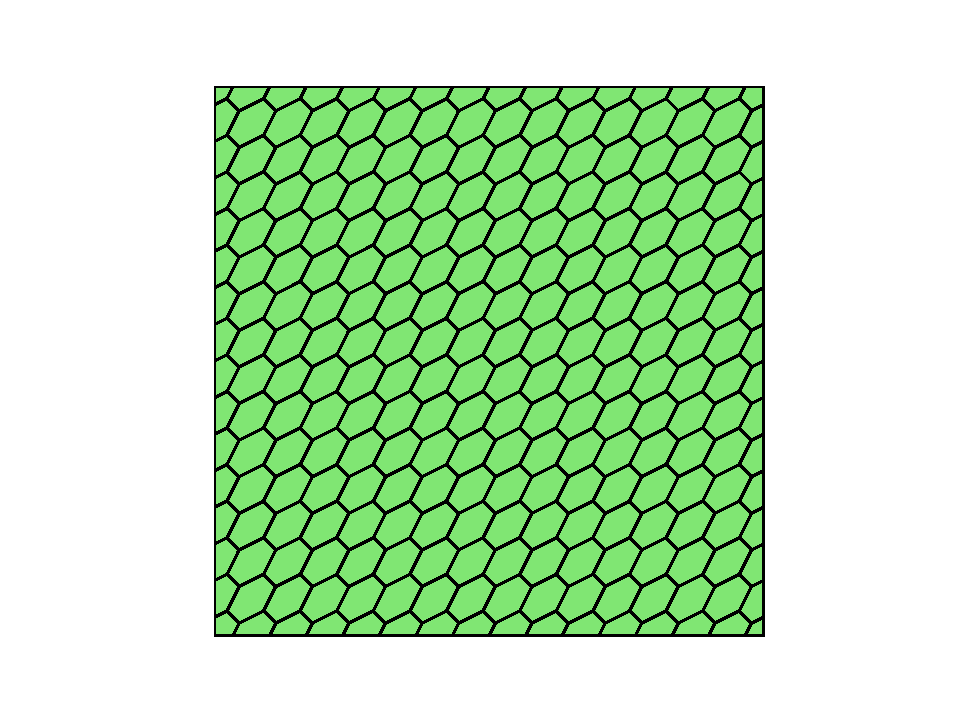
\includegraphics[width=4cm]{../figures/convex.pdf}
\captionsetup{font={small}}
\caption{Convex polygon mesh $\mathcal T_0$}
\end{minipage}%
\begin{minipage}[t]{0.49\linewidth}
\centering
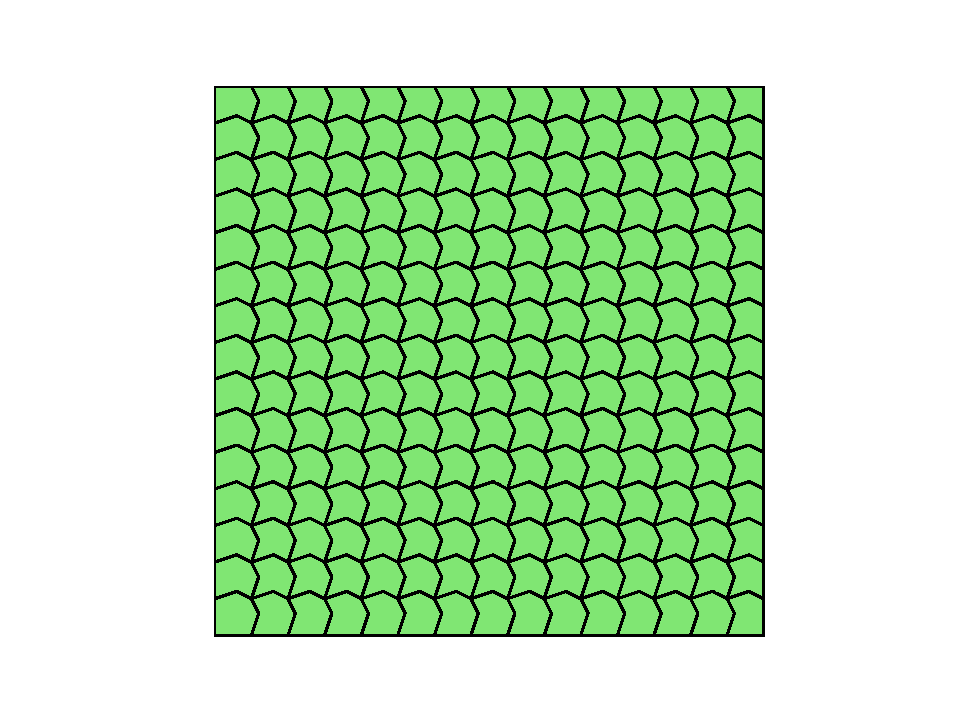
\includegraphics[width=4cm]{../figures/nonconvex.pdf}
\captionsetup{font={small}}
\caption{Non-convex polygon mesh $\mathcal T_1$}
\end{minipage}%
\centering
\end{figure}
\end{frame}

\begin{frame}
    \frametitle{数值结果}
We choose $k = 1, 2, 5$ in both SFNCVEM and SFCVEM.
The numerical results of the SFNCVEM on meshes $\mathcal T_0$ and $\mathcal T_1$
as follow. We can see that $\|u - Q_h u_h\|_0=O(h^{k+1})$ and $\|\nabla u -
Q_{h}\nabla_h u_h\|_0=O(h^{k})$, 
\begin{figure}[htbp]
\centering
\begin{minipage}[t]{0.49\linewidth}
\centering
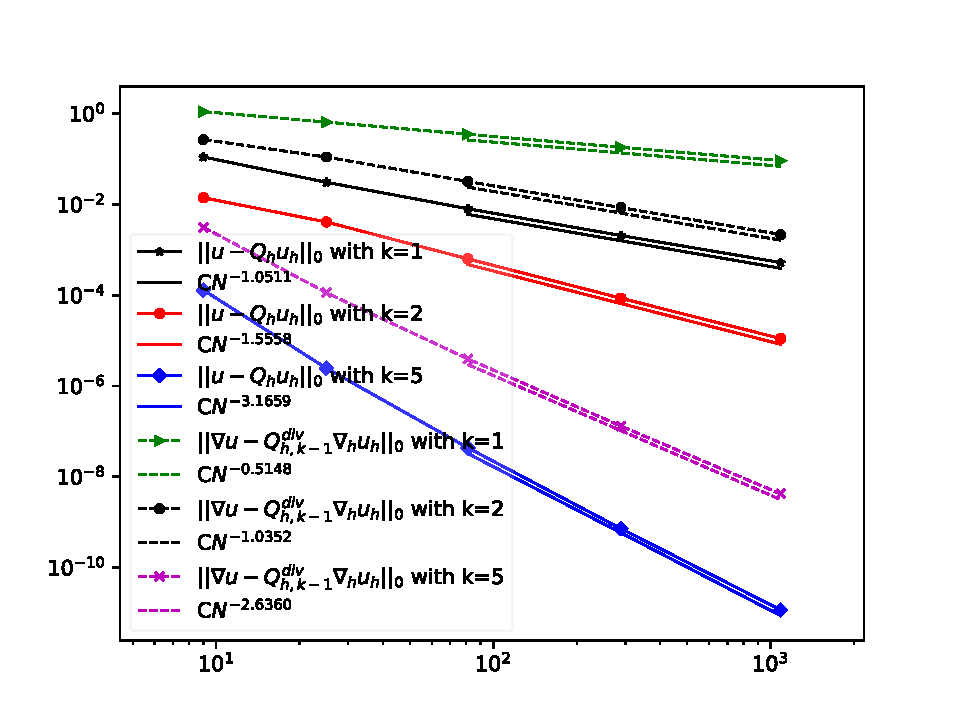
\includegraphics[width=5.5cm]{../figures/stabfree/ncvem_convex.pdf}
%\caption{Numberical result of example with $\mathcal T_0$.}
\end{minipage}%
\begin{minipage}[t]{0.49\linewidth}
\centering
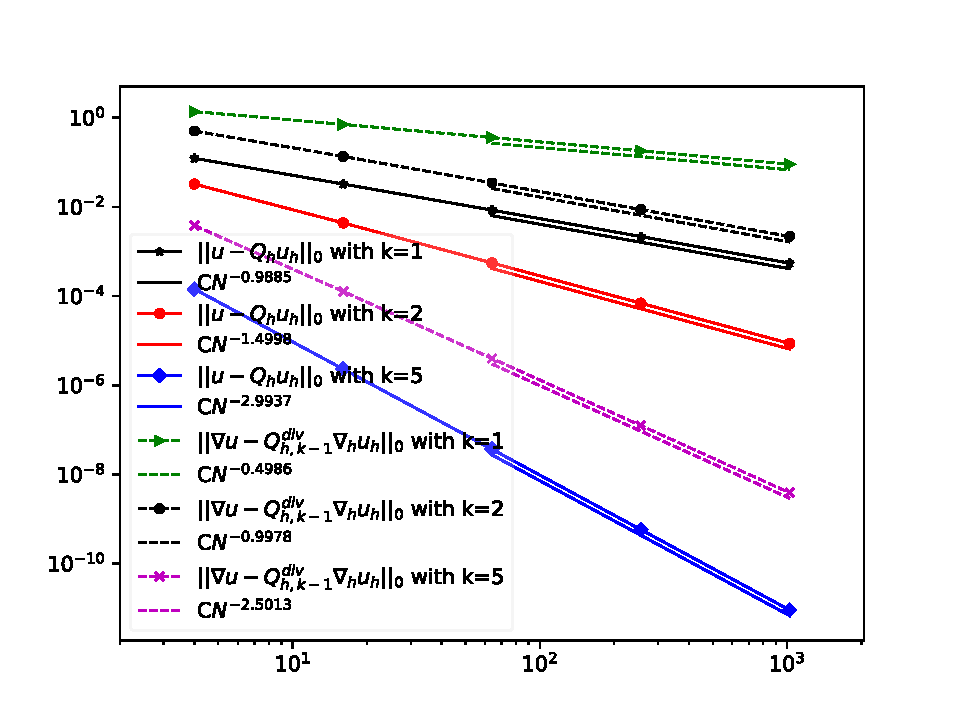
\includegraphics[width=5.5cm]{../figures/stabfree/ncvem_nonconvex.pdf}
%\caption{[Numberical result of example with $\mathcal T_1$].}
\end{minipage}%
\centering
\caption{Errors $\|u - Q_h u_h\|_0$ and $\|\nabla u - Q_{h}\nabla_h u_h\|_0$
of nonconforming VEM on
$\mathcal T_0$(left) and $\mathcal T_1$(right) with $k=1, 2, 5$.}
\label{fig:rate1}
\end{figure}


\end{frame}

\begin{frame}
    \frametitle{数值结果:收敛性}
And the numerical results of the SFCVEM are presented as follow. 
Again $\|u - Q_h u_h\|_0=O(h^{k+1})$ and $\|\nabla u - Q_{h}\nabla
u_h\|_0=O(h^{k})$. 

\begin{figure}[htbp]
\centering
\begin{minipage}[t]{0.49\linewidth}
\centering
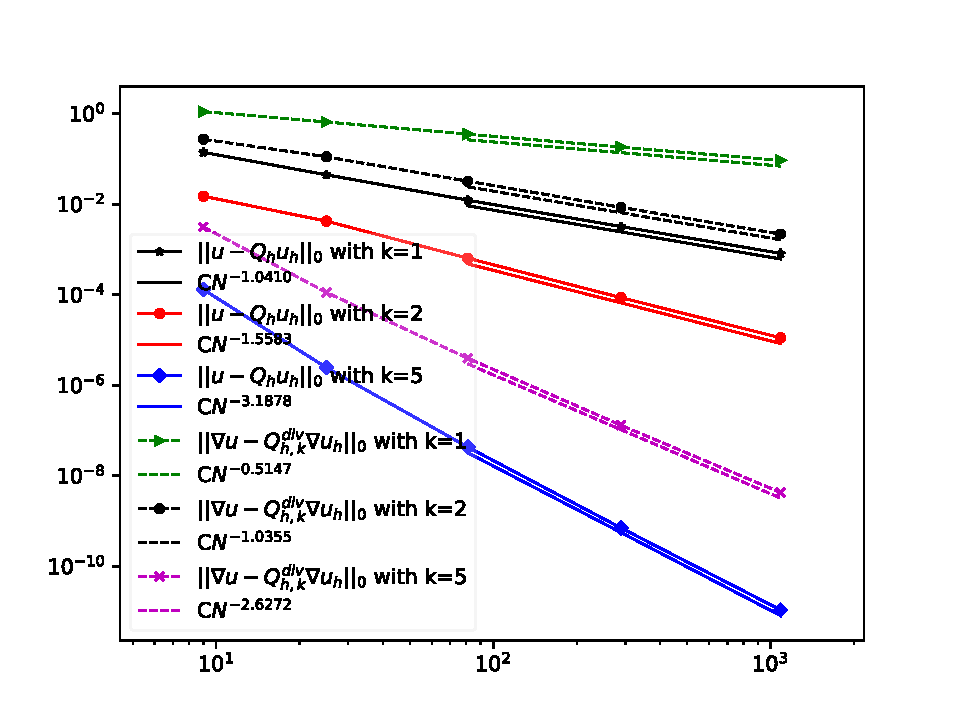
\includegraphics[width=5.5cm]{../figures/stabfree/cvem_convex.pdf}
%\caption{Numberical result of example with $\mathcal T_0$.}
\end{minipage}%
\begin{minipage}[t]{0.49\linewidth}
\centering
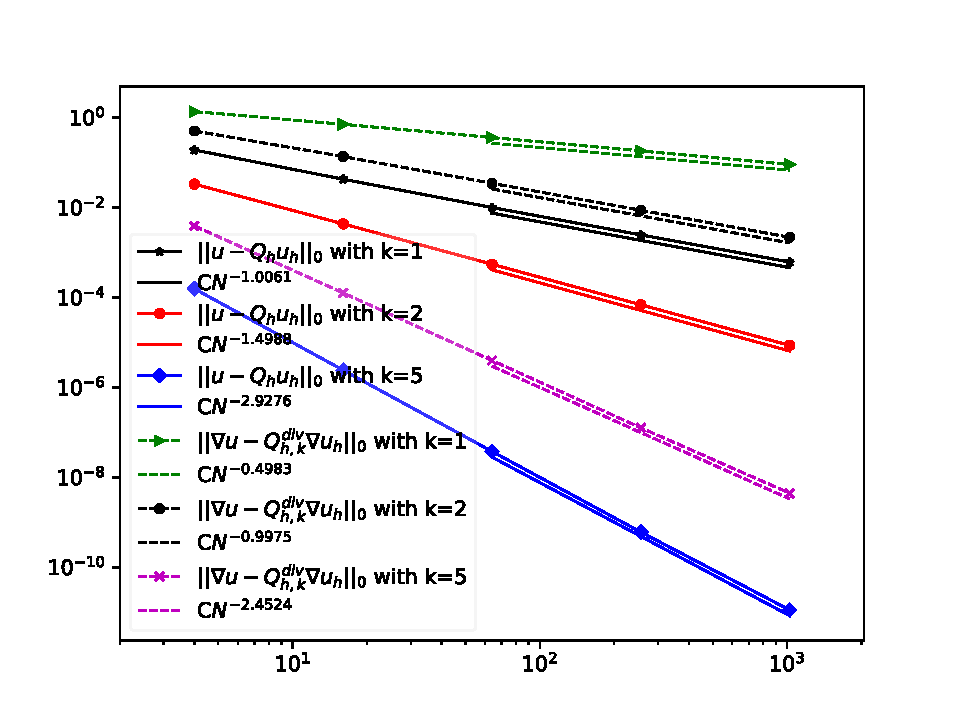
\includegraphics[width=5.5cm]{../figures/stabfree/cvem_nonconvex.pdf}
%\caption{[Numberical result of example with $\mathcal T_1$].}
\end{minipage}%
\centering
\caption{Errors $\|u - Q_h u_h\|_0$ and $\|\nabla u - Q_{h}\nabla u_h\|_0$
of conforming VEM on $\mathcal T_0$(left) and
$\mathcal T_1$(right) with $k=1, 2, 5$.}
\label{fig:rate2}
\end{figure}

\end{frame}

\begin{frame}
    \frametitle{数值结果:零特征值}
We construct three different hexagons shown as follow, and calculate the
eigenvalues of local stiffness matrices with $k=3$ for four virtual element
methods. 
% \begin{figure}[htbp]
% \centering
% \subfigure{\includegraphics[width=1.4in]{./figures/hexagon0.pdf}}
%     % \caption{Type I:5 tetrahedra}
% %%
% \subfigure{\includegraphics[width=1.4in]{./figures/hexagon1.pdf}}
%      %\caption{Type II: 24 tetrahedra}
% %%
% \subfigure{\includegraphics[width=1.2in]{./figures/hexagon2.pdf}}
%      %\caption{Trirectangular tetrahedron}
% %%
% \caption{The regular hexagon(Left), the quasi-regular hexagon generated by regular
%     hexagon with a small perturbation (Middle), 
% and the square with two hanging nodes (Right)}
%   \label{fig:hexagon0} %% label for entire figure
% \end{figure}
\begin{figure}[htbp]
\subfigure[Regular hexagon.]{
\begin{minipage}[t]{0.3\linewidth}
\centering
\includegraphics[width=1in]{../figures/stabfree/hexagon0.pdf}
\end{minipage}}%% 
\;\;% \quad
\subfigure[Quasi-regular hexagon generated by regular
    hexagon with a small perturbation.]
{\begin{minipage}[t]{0.3\linewidth}
\centering
\includegraphics[width=1in]{../figures/stabfree/hexagon1.pdf}
\end{minipage}}
\;\;% \quad
\subfigure[Square with two hanging nodes.]
{\begin{minipage}[t]{0.3\linewidth}
\centering
\includegraphics[width=0.9in]{../figures/stabfree/hexagon2.pdf}
\end{minipage}}
\caption{The regular hexagon(Left), the quasi-regular hexagon generated by regular
    hexagon with a small perturbation (Middle), 
and the square with two hanging nodes (Right).}
\end{figure}
\end{frame}

\begin{frame}
    \frametitle{Eigenvalues and condition numbers}
We also present the minimum
non-zero eigenvalue, the maximum eigenvalue and the condition number for the
local stiffness matrix on different hexagons, from
which we can see that these quantities are comparable for four virtual element
methods.
\only<1>{
\begin{table}[htbp]
\centering
\caption{Comparison of eigenvalues and condition numbers on the regular hexagon.}
\begin{tabular}{c|ccc}
\hline
\textbf{方法} & \textbf{最大特征值} & \textbf{最小特征值} & \textbf{条件数} \\ \hline
NCVEM & 975.5693189 & 0.309674737 & 3150.303211 \\ \hline
CVEM & 1012.488116 & 0.297206358 & 3406.683909 \\ \hline
SFNCVEM & 992.5956147 & 0.318932029 & 3112.248147 \\ \hline
SFCVEM & 1011.173331 & 0.298509692 & 3387.405362 \\
\hline
\end{tabular}
\end{table}
}
\only<2>{
\begin{table}[htbp]
\centering
\caption{Comparison of eigenvalues and condition numbers on the quasi-regular hexagon.}
\begin{tabular}{c|ccc}
\hline
\textbf{方法} & \textbf{最大特征值} & \textbf{最小特征值} & \textbf{条件数} \\ \hline
NCVEM   & 935.2883848 & 0.279027715 & 3351.955143 \\ \hline
CVEM    & 1014.672395 & 0.257370621 & 3942.456177 \\ \hline
SFNCVEM & 997.4831245 & 0.282126359 & 3535.589964 \\ \hline
SFCVEM  & 1047.876056 & 0.258970708 &
4046.311124 \\
\hline
\end{tabular}
\end{table}
}
\only<3>{
\begin{table}[htbp]
\centering
\caption{Comparison of eigenvalues and condition numbers on the square with two hanging nodes.}
\begin{tabular}{c|ccc}
\hline
\textbf{方法} & \textbf{最大特征值} & \textbf{最小特征值} & \textbf{条件数} \\ \hline
 NCVEM   & 941.8571938&	0.21069027	&4470.340249 \\ \hline
 CVEM    & 1046.755495&	0.200435123	&5222.4155 \\ \hline
 SFNCVEM & 986.5963357&	0.212761106	&4637.108513 \\ \hline
 SFCVEM  & 1061.651989&	0.202074633	&5253.761808 \\
\hline
\end{tabular}
\end{table}
}
\end{frame}


\section{时谐 Maxwell 方程的虚单元方法}
\begin{frame}
    \frametitle{时谐 Maxwell 方程界面问题}
\begin{minipage}[b]{0.6\linewidth}
    考虑如下时谐 Maxwell 方程:
    $$
    \left\{
    \begin{aligned}
        \mathbf{rot} \alpha \mathrm{rot} \boldsymbol{u} - \beta \boldsymbol{u} & = \boldsymbol{f} \quad
        \Omega\\
        u\times \mathbf{n} & = 0 \quad \partial\Omega
    \end{aligned}
    \right.
    $$
    其中 $\alpha > 0, \beta > 0$ 是分片常数:
    $$
    \alpha = \left\{
    \begin{aligned}
        \alpha_1 \quad & \text{in } \Omega^+,\\
        \alpha_2 \quad & \text{in } \Omega^-,
    \end{aligned}
\right.\quad
\beta = \left\{
\begin{aligned}
    \beta_1 \quad & \text{in } \Omega^+,\\
    \beta_2 \quad & \text{in } \Omega^-,
\end{aligned}
\right.
    $$
    界面条件为:
$$
\begin{aligned}
[\mathbf{u}\cdot\mathbf{t}]_{\Gamma} :=
(\mathbf{u}^+\cdot\mathbf{t}-\mathbf{u}^-\cdot\mathbf{t})|_{\Gamma} = 0\\
[\alpha \rot \mathbf{u}]_{\Gamma} := (\alpha \rot \mathbf{u}^+
- \alpha \rot \mathbf{u}^-)|_{\Gamma} = 0.
\end{aligned}
$$
\end{minipage}
\hfill
\begin{minipage}[b]{0.38\linewidth}
    \centering
    \begin{figure}[htpb]
        \centering
        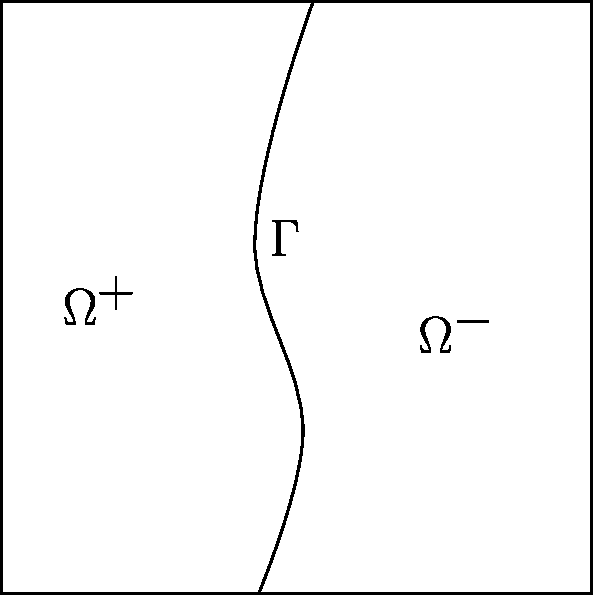
\includegraphics[width=0.8\textwidth]{../figures/interface_prob.pdf}
        \caption{界面问题求解区域.}
    \end{figure}
\end{minipage}
\end{frame}

\begin{frame}
  \frametitle{数值结果}
  \begin{minipage}[b]{0.6\linewidth}
    Set the domain and the interface geometry:
    $$
    \Omega = (-1, 1)\times(-1, 1), \quad \Omega^- = \{(x, y) : x^2+y^2 <
\left(\frac{\pi}{5}\right)^2\},\quad \Omega^+ = \Omega - \Omega^-,
    $$
    Consider the parameters $\alpha|_{\Omega^-} = \beta|_{\Omega^-} = 1, 
    \alpha|_{\Omega^+} = \beta|_{\Omega^+} = 10$, and the exact solution:
    \small{
    $$
    {u} = \left\{
        \begin{aligned}
        & - k_0(r_0^2 - x^2 - y^2)
        \begin{pmatrix}
        y\\
        x
        \end{pmatrix} \quad& \Omega^-, \\
        &-\frac{1}{10}
        k_1(r_0^2 - x^2 - y^2)(r_1^2 - x^2 - y^2)
        \begin{pmatrix}
        y\\
        x
        \end{pmatrix}& \Omega^+, \\
        \end{aligned} 
    \right.
    $$
}
    where $r_0 = \frac{\pi}{5}, r_1 = 1, k_1 = 20, k_0 = k_1(r_1^2-r_0^2).$
\end{minipage}
\hfill
\begin{minipage}[b]{0.38\linewidth}
    \centering
    \begin{figure}[htpb]
        \centering
        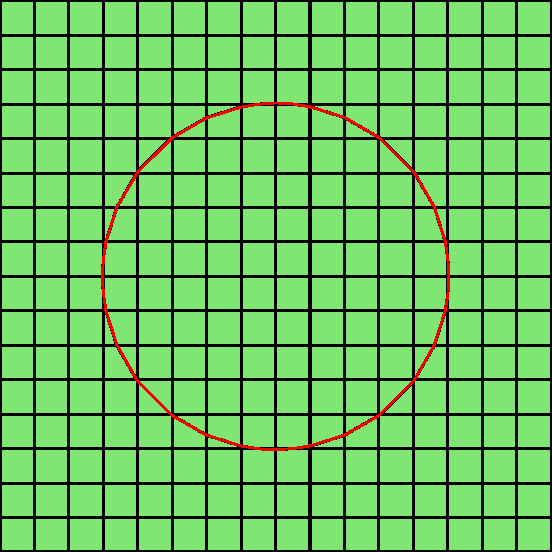
\includegraphics[width=0.6\textwidth]{../figures/maxwell/convergence_test.pdf}
        \caption{网格}
    \end{figure}
\end{minipage}

\end{frame}

\begin{frame}
    \frametitle{数值结果}
we can see that 
$\|\mathbf{u} - \Pi_h \mathbf{u}_h\|_{0,\Omega} = O(h), \|\rot \mathbf{u} -
\rot\mathbf{u}_h\|_{0,\Omega} = O(h)$ 
which is clearly optimal.
\begin{table}[!htp] 
\centering
\caption{Errors $||\mathbf{u} - \Pi_h \mathbf{u}_h||_{0,\Omega}$ and $||\rot
\mathbf{u} - \rot \mathbf{u}_h||_{0,\Omega}$ }
\label{tab:exm0}
\begin{tabular}[c]{|c|c|c|c|c|c|c|}\hline
$h$ & $1/8$ & $1/16$ & $1/32$ & $1/64$ 
\\\hline
$\|\mathbf{u} - \Pi_h{\mathbf{u}}_h \|_{0,\Omega}$ & 4.798e-01 & 2.192e-01 & 1.007e-01 & 4.761e-02 
\\\hline
Order & -- & 1.13 & 1.12 & 1.08 
\\\hline
$ \| \rot \mathbf{u} - \rot \mathbf{u}_h\|_{0,\Omega}$ & 1.155e+00 & 5.722e-01 & 2.726e-01 & 1.366e-01 
\\\hline
Order & -- & 1.01 & 1.07 & 1. 
\\\hline
\end{tabular}
\end{table} 


\end{frame}


\section{虚单元方法的实现}
\subsection{网格}
\begin{frame}
    \frametitle{数组化的半边数据结构}
    \begin{onlyenv}<1>

    \begin{columns}
       \column{0.4\textwidth}
       \centering
       \begin{figure}[htb]
           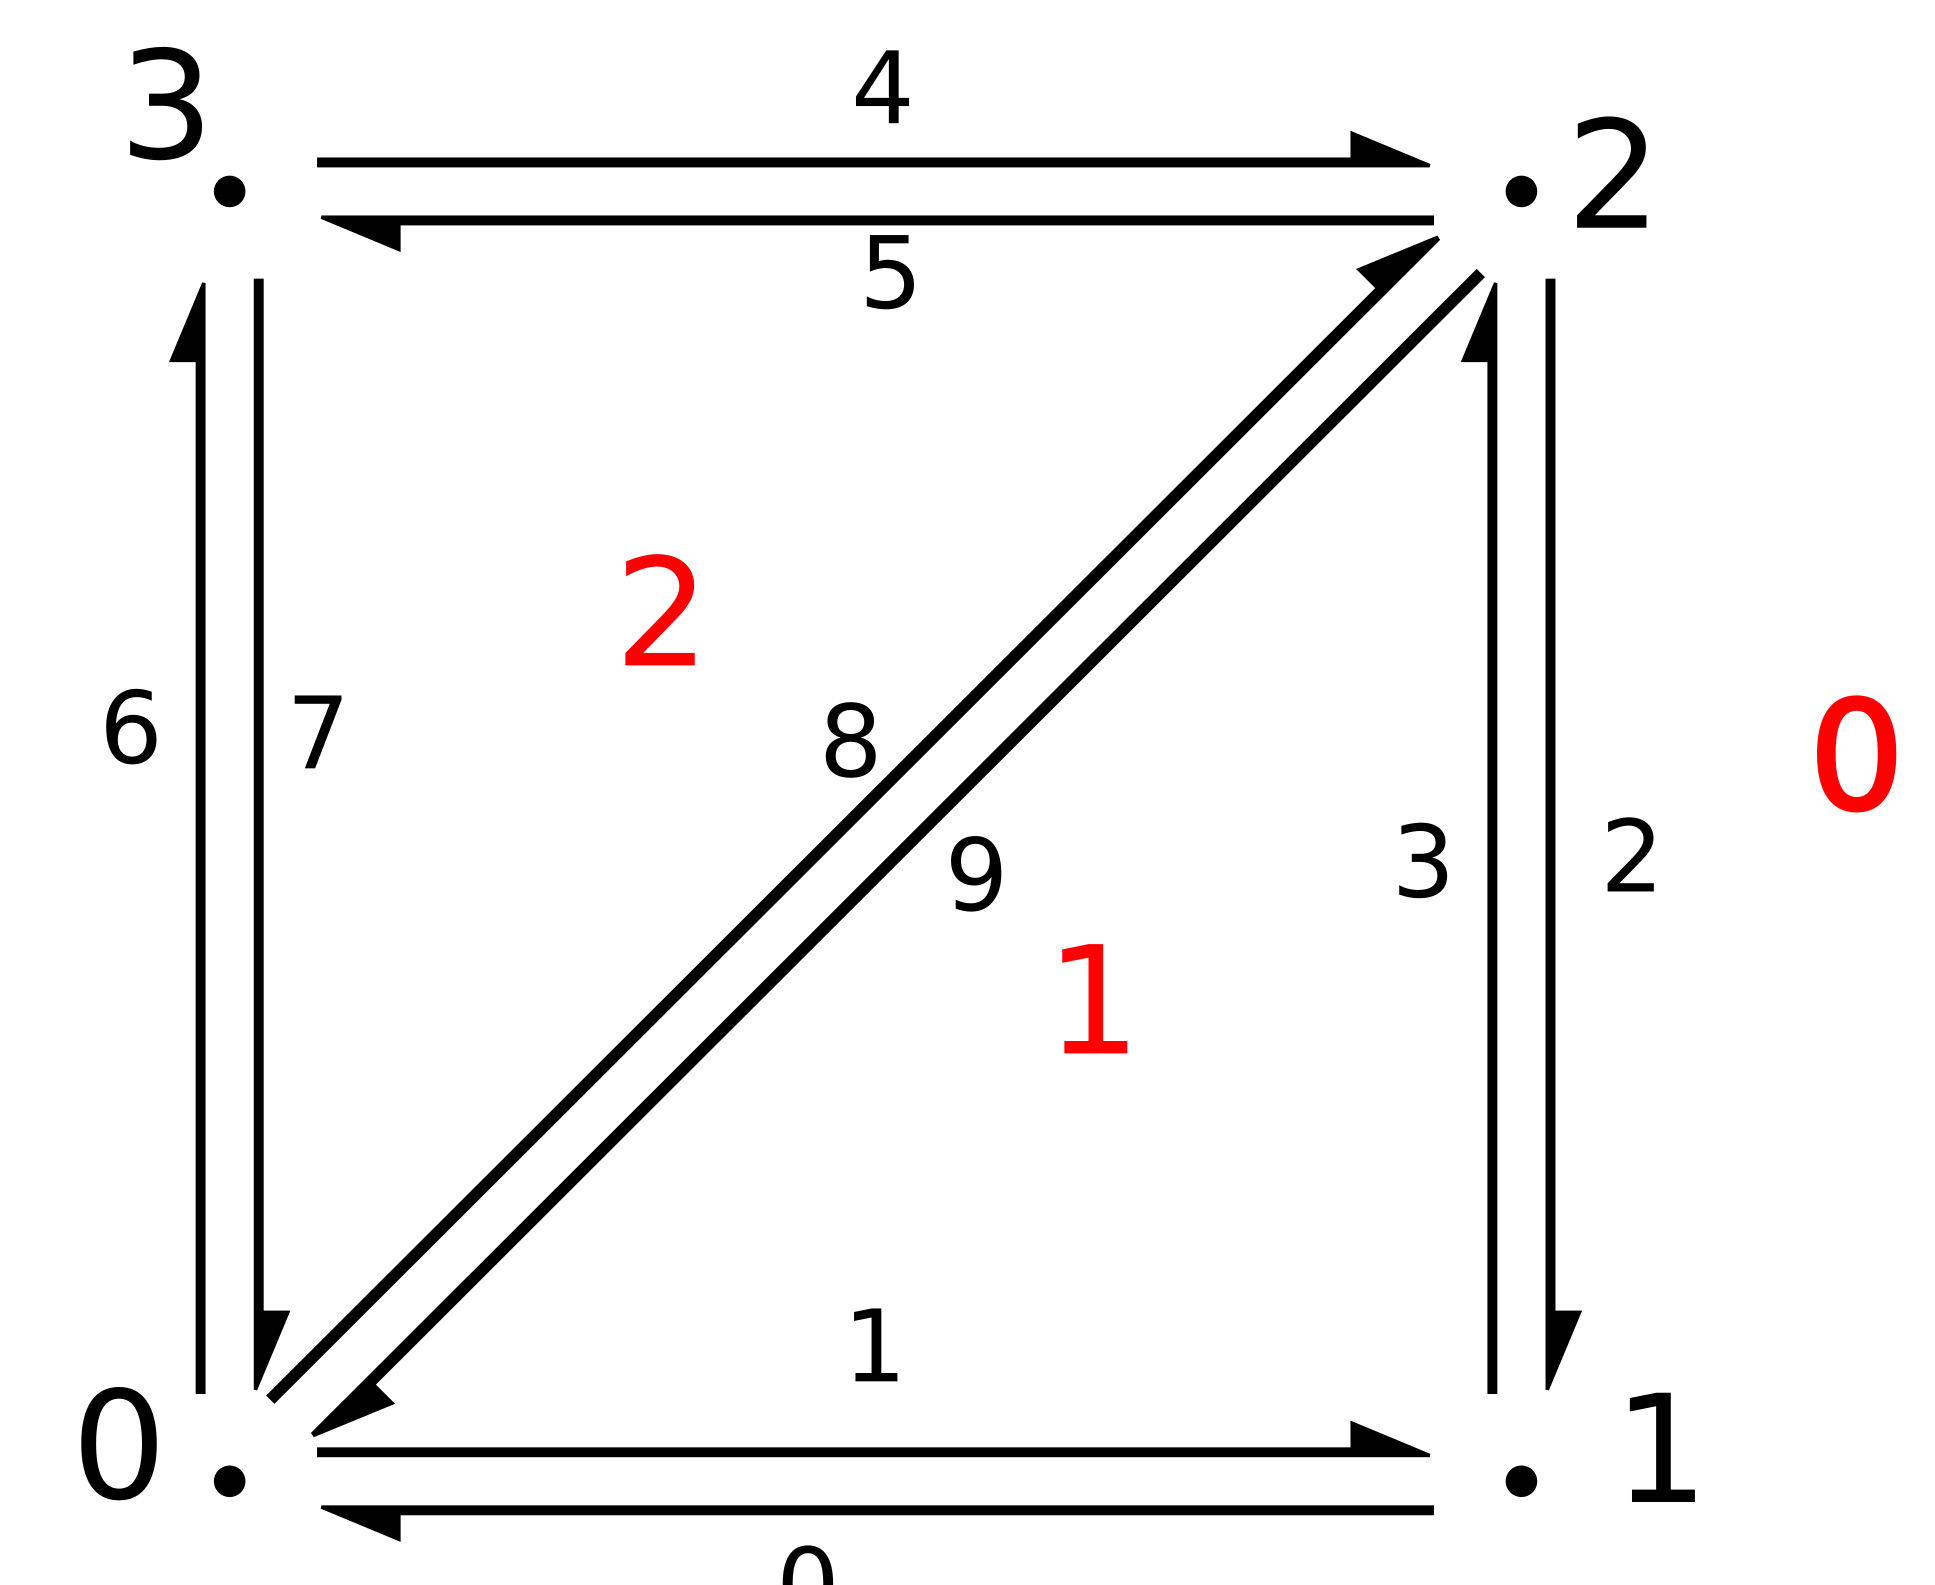
\includegraphics[scale=0.3]{../figures/cell.png}
         \caption{半边数据结构网格}
       \end{figure}
       \column{0.6\textwidth}
       \vspace{1pt}
       {\scriptsize
       \begin{tabular}{cccc}
           \hline
           半边 & 邻接信息 & 半边 & 邻接信息\\
           \hline
           \hline
           0 & [0, 0, 6, 2, 1] & 5 & [3, 2, 7, 8, 4]\\
           1 & [1, 1, 3, 9, 0] & 6 & [3, 0, 4, 0, 7]\\
           2 & [1, 0, 0, 4, 3] & 7 & [0, 2, 8, 5, 6]\\
           3 & [2, 1, 9, 1, 2] & 8 & [2, 2, 5, 7, 9]\\
           4 & [2, 0, 2, 6, 5] & 9 & [0, 1, 1, 3, 8]\\
           \hline
       \end{tabular}}
       \captionof{table}{半边邻接信息}
    \end{columns}
    \begin{table}[htb]
        \begin{minipage}[b]{.5\linewidth}
            \centering
            \begin{tabular}{cc}
                \hline
                起始半边 & [6, 9, 8]\\
                \hline
            \end{tabular}
            \caption{单元起始半边}
        \end{minipage}%
        \begin{minipage}[b]{.5\linewidth}
            \begin{tabular}{cc}
                \hline
                主半边 & [1, 3, 5, 7, 8]\\
                \hline
            \end{tabular}
            \caption{主半边}
        \end{minipage}
    \end{table}
    \end{onlyenv}
\end{frame}

\subsection{虚单元空间}
\begin{frame}
    \frametitle{缩放单项式空间}
\begin{minipage}[b]{0.55\linewidth}
For $\boldsymbol{\alpha} = (\alpha_0, \alpha_1) \in \mathcal{A}_k^2$, 
we can define the scaling monomial on $K$ as follows:
$$
m_{\boldsymbol{\alpha}}(x, y) = \frac{(x - x_K)^{\alpha_0}(y -
y_K)^{\alpha_1}}{h_K^{|\boldsymbol{\alpha}|}}
$$
where
\begin{itemize}
    \item $h_K$ denoting size of $K$. 
    \item $\boldsymbol{x_K} = (x_K, y_K)$ is the barycenter of $K$.
\end{itemize}
$\boldsymbol{m_k} = [m_0, m_1, m_2, \cdots, m_{n_k-1}], $
which forms a basis for the scalar space $\mathbb{P}_k(K)$.
\end{minipage}
\hfill
\begin{minipage}[b]{0.4\linewidth}
    \centering
    \begin{figure}[htpb]
        \centering
        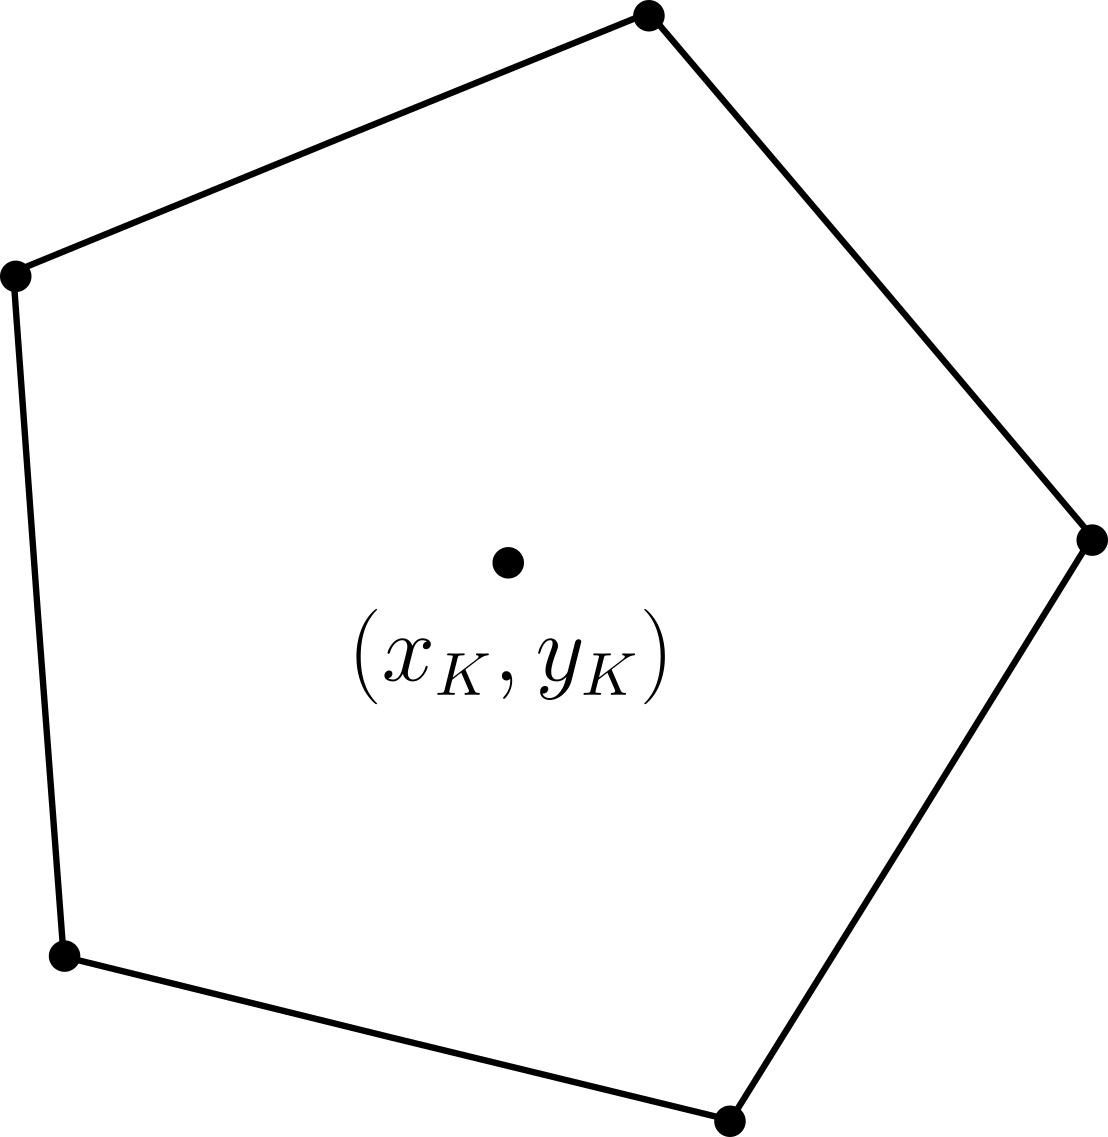
\includegraphics[width=0.8\textwidth]{../figures/polygon_K.png}
        \caption{Barycenter of $K$.}
    \end{figure}
\end{minipage}
\end{frame}

\begin{frame}
  \frametitle{缩放单项式求导}
  \begin{itemize}
      \item $\partial_x$ and $\partial_y$ is a linear map from $\mathbb{P}_k(K) \to
          \mathbb{P}_k(K)$.
          $$
          \partial_x m_{ \boldsymbol \alpha} = 
            \begin{cases}
            \frac{1}{h_K}\alpha_0 m_{\boldsymbol \alpha-(1, 0)} \quad & \alpha_0 > 0\\
            \quad 0 & \alpha_0 = 0
            \end{cases}
          $$
          define a matrix $P^x, P^y$:
          $$
          P_{\boldsymbol{\alpha\beta}}^x =
            \begin{cases}
            \frac{1}{h_K}\alpha_0 \quad & \boldsymbol \beta = \boldsymbol \alpha - (1, 0)\\
             0 & \mathrm{other}
         \end{cases},
            P^y_{ \boldsymbol{\alpha\beta}} =
            \begin{cases}
            \frac{1}{h_K}\alpha_1 \quad & \boldsymbol \beta = \boldsymbol \alpha - (0, 1)\\
             0 & \mathrm{other}
            \end{cases}
          $$
      \item the matrix representation of $\frac{\partial }{\partial
          \boldsymbol{t}}$ and $\frac{\partial^2 }{\partial
          \boldsymbol{t}\partial \boldsymbol{n}}$ is
          $$
          P^{\boldsymbol{t}} = t_0 P^x + t_1 P^y, \quad 
          P^{\boldsymbol{t}\boldsymbol{n}}= P^{\boldsymbol{t}}P^{\boldsymbol{n}}
          $$.
  \end{itemize}


\end{frame}

\begin{frame}
  \frametitle{缩放单项式的积分}
缩放单项式积分计算简单,因为缩放单项式是齐次函数,而
齐次函数在单元 $K$ 上的积分可以化简到单元边界上的积分。对于一个齐次函数 
$f$,其满足:
$$
f(k \bx) = k^q f(\bx)
$$
令等式两边同是对 $k$ 求导,可得
$$
\nabla f(k \bx)\cdot \bx = q k^{q-1} f(\bx)
$$
令 $k = 1$,可得
$$
f(\bx) = \frac{1}{q} \nabla f(\bx)\cdot \bx
$$
那么:
$$
\int_K f(\bx)d\bx = \frac{1}{q} \int_{K}
\nabla f(\bx)\cdot \bx d\bx
= -\frac{1}{q} \int_{K} f(\bx)\mathrm{div}{\bx}
\mathrm{d}\bx
+ \frac{1}{q} \int_{\partial K} f(\bx)\bx\cdot
\bn\mathrm{d}s
$$
注意 $\mathrm{div}{\bx} = n$,
所以我们可以把积分化简到单元边界上的积分:
$$
\int_K f(\bx)\mathrm{d}\bx = \frac{1}{q+n} \int_{\partial K}
f(\bx)\bx\cdot \bn\mathrm{d}s
$$
\end{frame}

\begin{frame}
  \frametitle{缩放单项式的积分}
上式对于任意 $n$ 维多面体 $K$,以及任意齐次函数 $f$
都成立,对于边界是平面的多面体,
边界上的积分还可以进一步化简,
令 $\mathcal{F}$ 为 $K$ 的边界面集合,对于 $F\in \mathcal{F}$,找到一个点
$\bx_F$ 在 $F$ 所在平面上,那么 
$(\boldsymbol{x-x}_F)\cdot \bn_F = 0$,
所以
$$
\int_{\partial K} f(\bx)\bx\cdot \bn
\mathrm{d}s = \sum_{F\in \mathcal{F}}
\int_{F} f(\bx)(\boldsymbol{x-x_F+x_F})\cdot \bn_F
\mathrm{d}s = \sum_{F\in \mathcal{F}}
\int_{F} f(\bx)\boldsymbol{x_F}\cdot \bn_F
\mathrm{d}s
$$

而缩放单项式 $m_{\boldsymbol{\alpha}}$
是一个齐次函数:
$$
m_{\boldsymbol{\alpha}}(k\bx) = k^{|\boldsymbol{\alpha}|}
m_{\boldsymbol{\alpha}}(\bx)
$$
所以其在单元上的积分可以化简到单元边界上的积分:
$$
\int_K m_{\boldsymbol{\alpha}}(\bx)\mathrm{d}\bx =
\frac{1}{|\boldsymbol{\alpha}|+n} \int_{\partial K}
m_{\boldsymbol{\alpha}}(\bx)\bx\cdot \bn
\mathrm{d}s
$$
\end{frame}

\begin{frame}
    \frametitle{缩放单项式的质量矩阵,刚度矩阵}
$m_{\boldsymbol{\alpha}}m_{\boldsymbol{\beta}} =
m_{\boldsymbol{\alpha+\beta}}$,所以缩放单项式的质量矩阵为
$$
\bM^{K}_{\boldsymbol{\alpha\beta}} = \int_K
m_{\boldsymbol{\alpha}}m_{\boldsymbol{\beta}}\mathrm{d}\bx =
\frac{1}{|\boldsymbol{\alpha}+\boldsymbol{\beta}|+n} \int_{\partial K}
m_{\boldsymbol{\alpha}}m_{\boldsymbol{\beta}}\bx\cdot \bn
\mathrm{d}s
$$
刚度矩阵为:
$$
\begin{aligned}
\bA^{K}_{\boldsymbol{\alpha\beta}} & = \int_K
\nabla m_{\boldsymbol{\alpha}}\cdot \nabla
m_{\boldsymbol{\beta}}\mathrm{d}\bx\\
& = 
\sum_{i=0}^{n-1} \int_K \partial_{x_i} m_{\boldsymbol{\alpha}}
\partial_{x_i} m_{\boldsymbol{\beta}}\mathrm{d}\bx
& = \sum_{i=0}^{n-1} P^{K, i}_{\boldsymbol{\alpha\gamma}}
\int_K m_{\boldsymbol{\gamma}}m_{\boldsymbol{\delta}}\mathrm{d}\bx
P^{K, i}_{\boldsymbol{\beta\delta}}
\end{aligned}
$$
即: $A^{K} = \sum_{i=0}^{n-1} \bP^{K, i}
\bM^{K} (\bP^{K, i})^T = \frac{1}{h_K^2}
\sum_{i=0}^{n-1} \bP^{i} \bM (\bP^{i})^T$。
同理,对于任意 $m>0$, 定义:
$$
A^{K, m}_{\boldsymbol{\alpha\beta}} = \int_K \nabla^m m_{\boldsymbol{\alpha}}
\cdot \nabla^m m_{\boldsymbol{\beta}}\mathrm{d}\bx
$$
\end{frame}

\end{document}



